\section{Analýza}
V tejto kapitole sa venujeme rozboru dostupných platforiem pre e-learning matematiky. 
Cieľom je identifikovať platformy, porovnať ich funkcie a odhaliť medzery, ktoré naša webová aplikácia môže vyplniť. 
Na trhu existuje široká škála platforiem pre e-learning rôznych matematických tém, 
z ktorých každá ponúka rôzne riešenia, funkcie a zameriava sa na odlišné cieľové skupiny.

\subsection{Brilliant.org}
Brilliant.org je online vzdelávacia platforma zameraná na interaktívne kurzy v oblastiach matematiky, vedy a počítačovej vedy.
Je navrhnutá tak, aby podporovala aktívne učenie prostredníctvom riešenia problémov a interaktívnych výziev, čím pomáha študentom rozvíjať kritické myslenie a logické schopnosti.
Platforma ponúka viac ako 60 kurzov, ktoré sú prispôsobené rôznym úrovniam znalostí, od začiatočníkov po pokročilých.

Medzi jej hlavné výhody patria interaktívne lekcie, ktoré sú navrhnuté tak, aby boli pútavé a vyžadovali aktívnu účasť študentov, čím zvyšujú efektivitu učenia.
Umožňuje tiež flexibilné a samostatné štúdium, čo je ideálne pre individuálne potreby. 
Platforma ponúka denné výzvy na rôzne témy, ktoré pomáhajú udržiavať študentov motivovaných a neustále zapojených do procesu učenia.
Nevýhodou je, že táto platforma je platená a dostupná len v anglickom jazyku, čo môže predstavovať prekážku pre niektorých študentov.
\cite{brilliant}
\subsection{Khan Academy}
Platforma Khan Academy ponúka bezplatné videokurzy a interaktívne cvičenia z rôznych oblastí matematiky, vrátane vysokoškolskej štatistiky a pravdepodobnosti.
Je vhodná pre študentov základných aj vysokých škôl. 
Medzi jej výhody patrí široká škála obsahu, jednoduché použitie a dostupnosť pre rôzne úrovne znalostí.
Dostupné zdroje k daným témam sú prehľadné a dobre štruktúrované.
Ponúka taktiež možnosť sledovania pokroku, získavania bodov a odznakov za splnené kapitoly, čím motivuje študentov k učeniu prostredníctvom gamifikácie\footnote{Gamifikácia je využitie herných prvkov a mechaník v nehernom prostredí s cieľom zvýšiť motiváciu, zapojenie a efektivitu používateľov.}.
Nevýhodou je, že je dostupná len v anglickom jazyku, čo môže byť pre niektorých študentov prekážkou. 
Používateľské rozhranie môže byť z dôvodu množstva obsahu pre niektorých používateľov neprehľadné, najmä ak sa na platforme nachádzajú prvýkrát. 
Napriek týmto nedostatkom je platforma považovaná za jeden z najlepších nástrojov na online vzdelávanie a sebarozvoj. \cite{khanacademy}
\subsection{Vieme matiku}
Najpopulárnejším slovenským portálom pre e-learning matematiky je Vieme matiku.
Táto platforma ponúka rôzne kurzy a cvičenia z matematiky pre žiakov základných a stredných škôl.
Medzi jej výhody patrí dostupnosť pre slovenských žiakov, široký výber tém, rôzne formy precvičovania,
do ktorých patrí grafické znázornenie úloh a možnosť sledovania pokroku.
Ponúka taktiež hravé prvky, ako sú grafické a zvukové efekty, ktoré môžu zvýšiť motiváciu žiakov.
Vyznačuje sa taktiež jednoduchým použitím a prehľadným rozhraním.
Nevýhodou je, že nie je dostupná pre študentov mimo Slovenska a je podporovaná len v slovenčine.
Platforma slúži na precvičovanie matematických úloh, ale neponúka zdroje pre samostatné štúdium alebo nápovedy. 
Zároveň, v prípade, že by sme chceli naplno využiť všetky jej funkcie, by bolo potrebné si zakúpiť licenciu. \cite{viemeto}
\subsection{Zhodnotenie}
Počas analýzy existujúcich vzdelávacích platforiem sme zistili, že na trhu chýbajú lokalizované a cenovo dostupné e-learningové riešenia pre stredoškolských a vysokoškolských študentov, ktoré by efektívne kombinovali gamifikáciu, interaktivitu a prehľadné rozhranie. 
Existujúce platformy, ako Brilliant.org a Khan Academy, ponúkajú kvalitné vzdelávacie materiály, ale ich dostupnosť je limitovaná anglickým jazykom a v prípade Brilliant.org aj plateným modelom. 
Vieme Matiku síce poskytuje lokalizovaný obsah, ale nezohľadňuje pokročilé potreby samostatného štúdia a je obmedzená na úzky okruh používateľov.
Analyzované platformy ukazujú širokú škálu prístupov, pričom mnohé sa zameriavajú na riešenie komplexných úloh alebo tradičné formy vzdelávania.
 Tieto prístupy však často nekladú dôraz na intuitívne osvojovanie matematických konceptov a podporu samostatného učenia. 
Tieto poznatky nám umožňujú identifikovať medzery a formulovať jasné požiadavky na vývoj novej aplikácie, ktorá by ponúkala lokalizovaný obsah, interaktívne učenie a dostupnosť pre rôzne cieľové skupiny.
\begin{table}[htbp]
\caption{Vzdelávacie platformy}
\label{vzdelavaciePlatformy}
\begin{tabularx}{\textwidth}{|X|X|X|X|}
\hline
\textbf{Platforma} & \textbf{Funkcie} & \textbf{Cieľová skupina} & \textbf{Cena} \\ \hline
Khan Academy & Videokurzy, cvičenia & Všetky úrovne & Bezplatná \\ \hline
Brilliant.org & Gamifikované kurzy & Stredné a Vysoké školy & Platená \\ \hline
Vieme Matiku & Online kurzy matematiky & Základné a Stredné školy & Čiastočne bezplatná \\ \hline
\end{tabularx}
\end{table}

\section{Použité technológie a knižnice}
V tejto kapitole sa podrobne venujeme technológiám a knižniciam, ktoré plánujeme
použiť na vývoj webovej aplikácie pre e-learning matematickej štatistiky a
pravdepodobnosti. Výber technológií je založený na princípoch flexibility,
kompatibility, bezpečnosti a aktívnej komunity vývojárov.


\subsection{Frontend}
Frontend je časť softvérového vývoja, ktorá sa zaoberá tým, čo používateľ vidí a s čím interaguje pri práci s aplikáciou alebo webovou stránkou. 
Ide o viditeľnú vrstvu aplikácie, ktorá zahŕňa všetky prvky používateľského rozhrania (\acrshort{ui}) a je priamo zodpovedná za používateľskú skúsenosť (\acrshort{ux}).

V kontexte nášho webového vývoja predstavuje frontend technológie a nástroje používané na tvorbu webových stránok, ktoré sú dostupné a vykresľované v internetových prehliadačoch. 
Zahŕňa návrh, implementáciu a optimalizáciu používateľského rozhrania tak, aby bolo esteticky príťažlivé, funkčné a dostupné na rôznych zariadeniach a platformách.
\subsubsection{HTML}
\acrfull{html} je značkovací jazyk používaný na tvorbu a štruktúrovanie obsahu webových stránok.
Umožňuje definovať rôzne prvky, ako sú nadpisy, odseky, obrázky či odkazy, čím určuje základnú kostru a vzhľad webovej stránky.
Napriek častým mylným predstavám, HTML nie je programovací jazyk, keďže neumožňuje vytvárať podmienené logické operácie alebo funkcie.
Jeho hlavnou úlohou je prezentácia a organizácia obsahu pre webové prehliadače. 
\cite{HTML}

\subsubsection{CSS}
\acrfull{css} \cite{css} je štýlovací jazyk používaný na definovanie vzhľadu a formátovania webových stránok. 
Umožňuje oddeliť vizuálnu prezentáciu od štruktúry obsahu definovanej v \acrshort{html}, čím zjednodušuje údržbu a aktualizáciu dizajnu.
Pomocou \acrshort{css} je možné nastaviť rôzne vizuálne vlastnosti, ako sú farby, písma, veľkosti, rozloženie prvkov a ďalšie aspekty dizajnu.
 Taktiež podporuje tvorbu responzívnych dizajnov, ktoré sa prispôsobujú rôznym zariadeniam a veľkostiam obrazoviek. 
 Moderné techniky, ako flexbox a grid, umožňujú presné rozmiestnenie a zarovnanie prvkov na stránke, čo je užitočné pri tvorbe komplexných rozložení.

\subsubsection{SCSS}
\acrfull{scss} je rozšírenie jazyka \acrshort{css}, ktoré pridáva pokročilé funkcie pre efektívnejšie štýlovanie webových stránok. 
\acrshort{scss} umožňuje používať premenné, vnáranie selektorov, mixiny, funkcie a operácie, čím zjednodušuje správu a údržbu štýlov.
 Vďaka svojim vlastnostiam podporuje modulárny prístup k tvorbe štýlov, čím zlepšuje čitateľnosť kódu a urýchľuje vývoj.

 \acrshort{scss} používa štandardnú \acrshort{css} syntax s doplnením nových funkcií, čo zabezpečuje spätnú kompatibilitu.
 Kód napísaný v \acrshort{scss} sa následne kompiluje do klasického \acrshort{css}, ktoré podporujú všetky moderné prehliadače. 
Tento proces zvyšuje flexibilitu vývoja a umožňuje tvorbu komplexných štýlových štruktúr.\cite{scss}
\subsubsection{JavaScript}
JavaScript \cite{JavaScript} je interpretovaný programovací jazyk ktorý umožňuje dynamickú interakciu s používateľom a zmeny obsahu webových stránok bez nutnosti ich opätovného načítania.

Podporuje objektovo orientované programovanie s triedami, objektmi a metódami, čo umožňuje tvorbu komplexných aplikácií. Vďaka svojej dynamickej povahe dokáže meniť obsah a štruktúru stránky počas jej behu.

Medzi jeho funkcie patrí funkcionálne programovanie, kde sú funkcie považované za prvotriedne objekty, a programovanie riadené udalosťami, ktoré umožňuje reagovať na interakcie používateľa, napríklad na kliknutia.

Je multiplatformový a podporuje rôzne zariadenia, ako sú počítače, smartfóny a tablety. Populárne knižnice a rámce ako jQuery, React, Angular a Vue výrazne uľahčujú vývoj aplikácií.

Medzi jeho vlastnosti patrí manipulácia s \acrfull{dom}, spracovanie udalostí, manipulácia s dátami a podpora asynchrónnych volaní na server pomocou techniky \acrfull{ajax}.
 Tieto vlastnosti z neho robia základný nástroj na tvorbu moderných webových aplikácií.
 \subsubsection{AJAX}
 AJAX (Asynchronous JavaScript and XML) je technológia, ktorá umožňuje webovým aplikáciám načítavať a odosielať dáta na pozadí bez nutnosti obnoviť celú stránku.
  Funguje na kombinácii známych technológií – HTML, CSS, JavaScript a XMLHttpRequest (alebo moderného fetch) – a výrazne zlepšuje interaktivitu a používateľskú skúsenosť. 
 AJAX sa využíva napríklad v ankete bez reloadu, našeptávačoch alebo moderných single-page aplikáciách.\cite{ajax}
\subsubsection{jQuery}
jQuery je open-source knižnica napísaná v JavaScripte, ktorá uľahčuje prácu s HTML dokumentom, manipuláciu s DOM, prácu s udalosťami, animáciami a technológiou AJAX.
 Bola vytvorená v roku 2006 s cieľom zjednodušiť vývoj v čase, keď neexistovala jednotná podpora v prehliadačoch.
  Aj napriek tomu, že je dnes považovaná za technicky zastaranú a dátovo náročnú, stále sa používa na mnohých weboch vďaka svojej jednoduchosti a veľkému množstvu dostupných pluginov.\cite{jquery}


 \subsubsection{java}
TypeScript \cite{TypeScript} je programovací jazyk vyvinutý spoločnosťou Microsoft, ktorý rozširuje možnosti JavaScriptu pridaním statického typovania a pokročilých objektovo orientovaných prvkov.
 Tým umožňuje vývojárom identifikovať chyby už počas vývoja, čo zvyšuje spoľahlivosť a udržiavateľnosť kódu.
  TypeScript je nadmnožinou JavaScriptu, čo znamená, že všetok platný kód v JavaScripte je kompatibilný s TypeScriptom.
   Po napísaní sa kód v TypeScripte transpiluje do štandardného JavaScriptu, ktorý je podporovaný vo všetkých moderných prehliadačoch. 
   Tento prístup umožňuje využívať výhody moderných programovacích techník pri zachovaní širokej kompatibility a flexibility, ktorú JavaScript ponúka.
\subsubsection{MathJax}
MathJax \cite{MathJax} je open-source\footnote{Open-source je softvér, ktorého zdrojový kód je voľne dostupný, môže byť používaný, upravovaný a distribuovaný kýmkoľvek.} JavaScriptový engine určený na zobrazovanie matematickej notácie, ako sú LaTeX, MathML a AsciiMath, v moderných webových prehliadačoch.
Je navrhnutý tak, aby konsolidoval pokroky vo webových technológiách do jednotnej platformy pre matematiku na webe, podporujúc hlavné prehliadače a operačné systémy, vrátane mobilných zariadení.
Používatelia nemusia inštalovať žiadne doplnky ani softvér; stačí, aby autor stránky zahrnul MathJax a matematický obsah do webovej stránky, a MathJax sa o zvyšok postará.


  \subsubsection{MathQuill}
  MathQuill \cite{mathquill} je open-source webový editor matematických výrazov navrhnutý tak, aby umožňoval jednoduché a estetické zadávanie matematiky priamo v prehliadači. 
  Umožňuje používateľom zadávať a zobrazovať matematické výrazy v známej vizuálnej forme pomocou syntaxe podobnej LaTeXu.

Je obľúbený v edukatívnych a interaktívnych webových aplikáciách, pretože poskytuje dynamické pole, v ktorom možno editovať matematické vzorce s okamžitým vizuálnym výstupom. 
MathQuill podporuje rôzne režimy – ako zobrazenie statických výrazov, interaktívne polia pre vstup používateľa alebo čítanie/zápis LaTeX kódu.
\subsubsection{ApexCharts}
ApexCharts\cite{apexcharts} je open-source JavaScriptová knižnica určená na vizualizáciu dát v podobe interaktívnych grafov.
 Poskytuje širokú škálu grafických typov a umožňuje ich jednoduchú integráciu do webových aplikácií s podporou populárnych frameworkov ako React, Angular či Vue. 
Vďaka svojej flexibilite, responzívnosti a podpore dynamických dát sa často využíva pri tvorbe analytických nástrojov a interaktívnych dashboardov.

\subsection{Backend}
Backend predstavuje časť softvérovej aplikácie, ktorá nie je priamo prístupná používateľom; ide o serverovú stranu v klient-server architektúre.
 Zodpovedá za hlavnú funkcionalitu aplikácie, vrátane spracovania webových požiadaviek, manipulácie s dátami a ich ukladania v databázach. Backend spolupracuje s frontendom, ktorý tvorí prezentačnú vrstvu aplikácie, s cieľom zabezpečiť komplexnú používateľskú skúsenosť. 
 Dáta generované na backende sú odosielané na frontend, kde sú prezentované používateľovi.
  Hoci sú často backend a frontend vyvíjané oddelenými tímami, hranica medzi nimi môže byť nejasná, čo vedie k prístupu známemu ako full-stack\footnote{Full-stack vývoj je proces, kde vývojár pracuje na frontende aj backende, teda na používateľskom rozhraní aj serverovej logike.} development, kde programátori pracujú na oboch stranách aplikácie.
   V minulosti backend pozostával prevažne z jednoduchých serverových skriptov, avšak s rozvojom webových technológií sa využívajú pokročilé frameworky umožňujúce dynamickú generáciu obsahu.
 Efektívny backendový kód je kľúčový pre optimalizáciu výkonu aplikácie, minimalizáciu zaťaženia servera a databázy, a zabezpečenie rýchlej odozvy pre používateľov. \cite{backend} 
 \subsubsection{API}
 \acrfull{api} je rozhranie, ktoré umožňuje jednej aplikácii komunikovať s inou aplikáciou alebo systémom. 
 Umožňuje vývojárom využívať už existujúce funkcionality bez toho, aby ich museli znova vytvárať, čím urýchľuje a zjednodušuje vývoj softvéru.
  \acrshort{api} definuje spôsob výmeny dát medzi klientom a serverom – napríklad keď mobilná aplikácia zobrazuje údaje o počasí získané zo servera.\cite{api}
 \subsubsection{REST}
 \acrshort{rest} \acrshort{api} (\acrfull{rest} acrfull{api}) je typ webového \acrshort{api}, ktorý umožňuje aplikáciám komunikovať medzi sebou pomocou štandardných \acrshort{http} protokolov. 
 REST API využíva jednoduché operácie ako čítanie, zápis, úprava a mazanie dát prostredníctvom \acrshort{url} adries a HTTP metód.

Jeho výhodou je jednoduchá štruktúra, škálovateľnosť a nezávislosť medzi klientom a serverom – klient nemusí poznať vnútornú logiku servera a server nemusí vedieť nič o klientskom rozhraní.
 REST API je široko používané pri vývoji moderných webových a mobilných aplikácií, pretože umožňuje flexibilnú a efektívnu výmenu dát.
\subsubsection{CORS}
CORS (Cross-Origin Resource Sharing) predstavuje mechanizmus, ktorý umožňuje realizáciu HTTP požiadaviek medzi rôznymi doménami (tzv. cross-origin požiadavky).
 Ide o spôsob, ako prehliadače môžu bezpečne vykonávať požiadavky na zdroje umiestnené na iných serveroch, než odkiaľ pochádza pôvodná webová stránka. 
 V minulosti takéto požiadavky bránila politika rovnakého pôvodu (same-origin policy), ktorá obmedzovala skripty bežiace v prehliadači výhradne na komunikáciu so serverom tej istej domény.

Mechanizmus CORS funguje tak, že server explicitne definuje, kto môže vytvárať požiadavky na jeho \acrshort{api}
, aké typy požiadaviek sú povolené a aké HTTP metódy sú podporované.
 Toto sa realizuje prostredníctvom špeciálnych HTTP hlavičiek, ktoré umožňujú prehliadaču určiť, či konkrétna požiadavka medzi rôznymi doménami môže byť bezpečne vykonaná.
 \cite{CORS}
\subsubsection{Node.js}
Node.js je runtime\footnote{Runtime prostredie je prostredie poskytujúce aplikácii všetky potrebné zdroje, knižnice a služby, ktoré sú potrebné na jej spustenie a beh.}
prostredie umožňujúce použitie JavaScriptu na strane servera, pričom využíva flexibilitu a jednoduchosť tohto programovacieho jazyka.
 Výhodou JavaScriptu sú jeho pokročilé koncepty ako „first-class functions“ (funkcie prvej triedy) a closures, ktoré umožňujú vytváranie efektívnych webových aplikácií. 
 Hoci JavaScript býva kritizovaný za nespoľahlivosť, táto kritika vyplýva predovšetkým zo zvláštností \acrshort{dom}-u v prehliadačoch, nie zo samotného jazyka.
 \subsection{Databázové systémy}
 Databázový systém je softvérové riešenie, ktoré slúži na efektívne uchovávanie, správu a vyhľadávanie dát. 
 Umožňuje vytvárať databázy, ktoré obsahujú štruktúrované dáta usporiadané v tabuľkách, a poskytuje nástroje na ich úpravu, triedenie, filtrovanie a prezentáciu.
 
 Databáza samotná je organizovaný súbor údajov, často rozdelený do tabuliek, ktoré spolu súvisia a medzi ktorými môžu byť definované vzťahy. 
 Cieľom databázového systému je zabezpečiť integritu, konzistenciu a dostupnosť dát, pričom používateľ môže s dátami pracovať pomocou formulárov, dotazov či zostáv.\cite{databazovesystemy}
 
 \subsubsection{SQL}
 \acrfull{sql} je jazyk navrhnutý na prácu s dátami v relačných databázach, pričom umožňuje ich efektívne ukladanie, organizáciu a získavanie.
 V \acrshort{sql} sa údaje ukladajú do tabuliek, ktoré fungujú ako dvojrozmerné štruktúry zložené z riadkov a stĺpcov. 
 Každá tabuľka predstavuje určitý typ objektu (napr. zákazníci, produkty) a každý riadok v tabuľke predstavuje jeden záznam s konkrétnymi údajmi.
 
 Pomocou dotazov (queries) je možné z databázy získať presne tie údaje, ktoré používateľ potrebuje – napríklad filtrovať podľa podmienok, zoskupovať dáta alebo ich spájať z viacerých tabuliek.
 Dotazy sú základom práce s \acrshort{sql} a umožňujú analyzovať, transformovať a prezentovať uložené informácie v požadovanej forme.\cite{sql}
 
 \subsubsection{PostgreSQL}
 PostgreSQL je pokročilý open-source objektovo-relačný databázový systém (\acrshort{ordbms}), ktorý kombinuje tradičné vlastnosti relačných databáz so schopnosťou pracovať s objektovo orientovanými prvkami. 
 To znamená, že okrem práce s tabuľkami a vzťahmi (typických pre \acrfull{rdbms}) podporuje aj vlastné dátové typy, dedičnosť, či ukladanie komplexných štruktúr, ako sú napríklad JSON či geografické dáta.
 
 Ako \acrshort{ordbms}, PostgreSQL umožňuje definovať vlastné funkcie, procedúry a typy, čím ponúka vysokú mieru prispôsobiteľnosti pre náročné aplikácie. 
 Je navrhnutý s dôrazom na integritu dát, rozšíriteľnosť a štandardy \acrshort{sql}, a preto je široko používaný v podnikových riešeniach, výskumných systémoch aj moderných webových aplikáciách.\cite{postgre}
 \subsubsection{DBDiagram}
 dbdiagram.io je bezplatný online nástroj, ktorý umožňuje vývojárom a dátovým analytikom jednoducho vytvárať diagramy a databázových štruktúr pomocou jednoduchého textového zápisu.
 Jeho hlavnou výhodou je schopnosť rýchlo a efektívne navrhovať a vizualizovať databázové schémy, čo uľahčuje plánovanie a komunikáciu v tímoch.
 Používatelia môžu definovať tabuľky, stĺpce a vzťahy medzi nimi v jednoduchom jazyku, pričom nástroj automaticky generuje zodpovedajúci diagram.
 Okrem toho dbdiagram.io podporuje import a export SQL skriptov, čo umožňuje integráciu s existujúcimi databázami a uľahčuje migráciu alebo dokumentáciu databázových štruktúr.
 Vďaka týmto funkciám je dbdiagram.io obľúbeným nástrojom pre rýchly návrh databáz a spoluprácu na databázových projektoch.
 \subsection{Framework}
 Framework je softvérová platforma poskytujúca vývojárom preddefinovanú štruktúru a nástroje, ktoré urýchľujú a zjednodušujú proces vývoja aplikácií.
 Existujú rôzne typy frameworkov podľa oblasti použitia, napríklad webové, desktopové či mobilné.
 Používanie frameworkov prináša výhody ako rýchlejší vývoj, lepšiu kvalitu kódu a štandardizáciu práce vývojárov. \cite{framework}
 \subsubsection{Frontendové frameworky}
 Frontend framework je špecializovaný typ frameworku určený na vývoj používateľských rozhraní webových aplikácií.
 Na rozdiel od všeobecných frameworkov, ktoré môžu pokrývať celý vývojový cyklus aplikácie, frontend framework sa sústreďuje výhradne na klientskú časť – teda na to, čo používateľ vidí a s čím interaguje v prehliadači.
 Poskytuje nástroje a štruktúru na organizáciu komponentov, správu stavu aplikácie a manipuláciu s \acrshort{dom}-om, čím umožňuje tvorbu dynamických, responzívnych a udržiavateľných rozhraní.
 \subsubsection{Rozdiel medzi CSS a JavaScript (JS) frameworkami}
 \begin{itemize}
  \item CSS frameworky (napr. Bootstrap, Tailwind CSS, Materialize) sú zamerané na vizuálnu stránku webu – poskytujú hotové štýly, rozloženia, komponenty (tlačidlá, formuláre, mriežky), ktoré zjednodušujú tvorbu konzistentného a estetického dizajnu. Ide predovšetkým o „vzhľad“ aplikácie.
  \item JS frameworky (napr. React, Angular, Vue.js) naopak poskytujú funkčnú logiku a štruktúru aplikácie. 
  Umožňujú pracovať s dátami, dynamicky meniť obsah stránky bez opätovného načítania (tzv. \acrshort{spa}), pracovať s API a definovať správanie komponentov.\cite{feframework}
\end{itemize}
\subsubsection{Angular}
Angular je open-source framework vyvinutý spoločnosťou Google, určený na tvorbu dynamických a responzívnych webových aplikácií.
Umožňuje vývojárom vytvárať aplikácie s bohatou funkcionalitou prostredníctvom komponentovo orientovanej architektúry, ktorá podporuje opätovné použitie kódu a zjednodušuje údržbu aplikácií.
Angular využíva TypeScript, nadmnožinu JavaScriptu, ktorá pridáva statické typovanie a ďalšie funkcie zlepšujúce vývojový proces. 
Medzi kľúčové vlastnosti Angularu patrí obojsmerná väzba dát, ktorá synchronizuje model a zobrazenie, a modulárny systém, ktorý umožňuje rozdelenie aplikácie na menšie, ľahko spravovateľné časti.
Angular tiež obsahuje nástroje na správu formulárov, komunikáciu so serverom a smerovanie, čo umožňuje vytvárať komplexné aplikácie s minimálnym úsilím. \cite{angular}

\subsubsection{RxJs}
\acrshort{rxjs} \acrfull{rxjs} je knižnica určená na reaktívne programovanie, ktorá umožňuje efektívne spracovanie asynchrónnych a udalostne založených dátových tokov pomocou tzv. observables. 
Tieto observables predstavujú prúdy dát (napr. kliknutia, HTTP odpovede), ktoré môžu byť pozorované a spracovávané rôznymi operátormi ako map, filter či reduce.

RxJS umožňuje prehľadnejšie a konzistentnejšie riadiť komplexné interakcie v aplikáciách, najmä tam, kde dochádza k častým zmenám stavu alebo udalostiam v čase.
Využíva sa najmä v moderných frontend frameworkoch, ako je Angular, kde zjednodušuje prácu s dátami a udalosťami.\cite{rxjs}
\subsubsection{Backendové frameworky}
Back-end framework je softvérový nástroj, ktorý uľahčuje vývoj serverovej časti webovej aplikácie. 
Poskytuje štruktúru, komponenty a funkcie potrebné na spracovanie požiadaviek, prácu s databázou, autentifikáciu a ďalšie serverové operácie. 
Cieľom back-end frameworku je zefektívniť vývoj, zabezpečiť konzistentnosť kódu a podporiť štandardizované riešenia. 
Rôzne frameworky (napr. Django, Spring, Laravel, Ruby on Rails, Express) sa líšia podľa náročnosti projektu, škálovateľnosti, dokumentácie a vhodnosti pre začiatočníkov či veľké podnikové aplikácie.\cite{backendframework}

Node.js tak využíva práve dobre definované vlastnosti JavaScriptu, ktoré umožňujú vytvárať vysoko výkonné platformy pre webové aplikácie.\cite{nodejs}
\subsubsection{Express.js}
Express je JavaScriptový framework fungujúci ako ľahká nadstavba nad Node.js, ktorý zjednodušuje tvorbu webových aplikácií a \acrshort{api}.
Zatiaľ čo Node.js poskytuje základné prostredie pre spúšťanie JavaScriptu na serveri, Express pridáva štruktúru a pomáha vývojárom vyhnúť sa opakovanému a zdĺhavému písaniu nízkoúrovňového kódu. 
Express je teda nástroj, ktorý zjednodušuje a zrýchľuje vývoj tým, že poskytuje vyššiu úroveň abstrakcie oproti základným funkciám dostupným v čistom Node.js.

Jeho minimalistická architektúra ponúka veľkú mieru flexibility – vývojári nie sú nútení dodržiavať presne stanovenú štruktúru projektu, no zároveň majú k dispozícii nástroje na efektívne spracovanie HTTP požiadaviek, tvorbu routovacích pravidiel a využívanie middleware vrstiev. 
Express umožňuje jednoduché vytváranie \acrshort{rest}ful \acrshort{api} a dynamických webových aplikácií.
Pre svoju jednoduchosť, rozsiahlu dokumentáciu a silnú komunitu patrí medzi najpopulárnejšie riešenia pre serverovú časť aplikácií postavených na JavaScripte.\cite{express}\cite{backendframework}
\subsection{UI a UX}
Používateľské rozhranie predstavuje vizuálnu časť digitálneho produktu, s ktorou používateľ priamo interaguje. 
Zahŕňa prvky ako tlačidlá, ikony, typografiu a farebné schémy. 
Cieľom UI dizajnu je vytvoriť esteticky príjemné a funkčné prostredie, ktoré uľahčuje používateľovi navigáciu a interakciu s produktom.

Používateľský zážitok sa zameriava na celkovú skúsenosť používateľa pri interakcii s produktom alebo službou. 
Ide o to, ako intuitívne a efektívne dokáže používateľ dosiahnuť svoje ciele. 
UX dizajn zahŕňa analýzu potrieb používateľov, návrh informačnej architektúry, prototypovanie a testovanie, s cieľom zabezpečiť, aby bol produkt nielen funkčný, ale aj príjemný na používanie.

Hoci sú UI a UX odlišné disciplíny, úzko spolupracujú s cieľom vytvoriť digitálne produkty, ktoré sú nielen vizuálne atraktívne, ale aj používateľsky prívetivé a efektívne.\cite{uiux}
\subsubsection{Figma}
Figma je cloudová platforma na návrh a prototypovanie používateľských rozhraní pre webové a mobilné aplikácie. 
Umožňuje tímovú spoluprácu v reálnom čase prostredníctvom webového prehliadača alebo desktopovej aplikácie. Podporuje vektorové ilustrácie, interaktívne prototypy a dizajnové systémy.
 Všetky projekty sú uložené v cloude, čo zjednodušuje prístup a zdieľanie. \cite{figma}
 \subsubsection{Material UI}
 Angular Material UI je oficiálna knižnica komponentov pre Angular, ktorá implementuje dizajnové princípy Material Design od spoločnosti Google. 
 Poskytuje predpripravené a prispôsobiteľné komponenty, ako sú tlačidlá, formuláre, tabuľky či navigačné panely, ktoré umožňujú vývojárom rýchlo vytvárať moderné, responzívne a esteticky príjemné používateľské rozhrania.
  Angular Material UI podporuje integráciu s Angular frameworkom a zabezpečuje konzistentný dizajn a vysokú úroveň použiteľnosti v rámci aplikácií. \cite{materialUI}

\subsection{Gamifikácia}
Gamifikácia je aplikácia herných prvkov a princípov v neherných kontextoch s cieľom zvýšiť angažovanosť a motiváciu jednotlivcov pri vykonávaní určitých aktivít.
 Tento prístup sa využíva v rôznych oblastiach, ako sú vzdelávanie, marketing, podnikanie a osobný rozvoj.
Vo vzdelávacom prostredí to znamená implementáciu mechanizmov, ako sú zbieranie bodov, získavanie odmien, porovnávanie sa s ostatnými či postupovanie na vyššie úrovne, aby sa proces učenia stal interaktívnejším a pútavejším. 
\subsubsection{Gamifikácia v e-learningu}
Gamifikácia v e-learningu zahŕňa integráciu herných prvkov, ako sú body, odznaky, rebríčky a úrovne, do vzdelávacích online prostredí s cieľom zvýšiť motiváciu a angažovanosť študentov.
 Podľa príspevku v zborníku z medzinárodnej vedeckej konferencie "Vzdělávání dospělých 2021" \cite{gamifikacia} je gamifikácia efektívnym nástrojom na podporu aktívneho učenia, pretože využíva prirodzenú ľudskú tendenciu k hre a súťaživosti.
  Implementácia herných mechanizmov v e-learningových kurzoch môže viesť k zlepšeniu zapojenia študentov, zvýšeniu ich motivácie a následne k lepším vzdelávacím výsledkom.

\subsection{Server}
Server je centrálny počítač v sieti, ktorý poskytuje služby a zdroje iným zariadeniam – tzv. klientom. 
Umožňuje uchovávať a sprístupňovať dáta, spúšťať aplikácie, spracovávať požiadavky používateľov alebo poskytovať webové stránky či e-mailové služby.
 Môže ísť o fyzický počítač alebo virtuálny stroj a jeho konkrétna funkcia závisí od typu – napríklad súborový, databázový, aplikačný alebo webový server. 
 Správne nastavený server je základom spoľahlivej a bezpečnej IT infraštruktúry.\cite{server}
\subsubsection{NGINX}
Nginx\cite{nginx} je výkonný a spoľahlivý webový a reverzný proxy server, ktorý je navrhnutý na efektívne spracovanie veľkého množstva súčasných pripojení pri minimálnom využití systémových zdrojov. 
Najčastejšie sa používa na poskytovanie statického obsahu, ako sú HTML, CSS, JavaScript alebo obrázky, a zároveň ako sprostredkovateľ medzi klientom a backend aplikáciou, čím preposiela požiadavky na servery bežiace napríklad v Node.js alebo PHP. 
Nginx dokáže tiež rozdeľovať záťaž medzi viaceré servery, čím zabezpečuje vyššiu dostupnosť a škálovateľnosť aplikácií, a môže slúžiť ako cache server pre rýchlejšie doručovanie často používaného obsahu.
 Vďaka svojej asynchrónnej architektúre a podpore moderných protokolov, ako sú \acrshort{http}/3 a \acrshort{tls}, je ideálnym riešením pre hosting moderných webových aplikácií s vysokými nárokmi na výkon.
\subsubsection{Docker}
Docker je open-source platforma, ktorá umožňuje vývoj, distribúciu a správu aplikácií pomocou tzv. kontajnerov. 
Kontajner je ľahké a izolované prostredie, ktoré obsahuje všetko potrebné na beh aplikácie – vrátane kódu, knižníc, runtime prostredia a nastavení.

Vďaka tomu môže aplikácia bežať rovnakým spôsobom na rôznych miestach, napríklad na vývojárskom počítači, v testovacom prostredí aj na produkčnom serveri. 
Docker využíva virtualizáciu na úrovni operačného systému, čo mu umožňuje spúšťať viacero kontajnerov efektívne a s nízkymi nárokmi na systémové prostriedky.\cite{docker}
\subsection{GIT}
Git je distribuovaný systém na správu verzií, ktorý umožňuje sledovať a zaznamenávať zmeny v súboroch počas vývoja softvéru.
 Umožňuje viacerým vývojárom pracovať súčasne na tom istom projekte, pričom každá kópia projektu obsahuje úplnú históriu zmien. 
 Git je známy svojou rýchlosťou, flexibilitou a podporou nelineárnych pracovných tokov. 
Je open-source, bezplatný a vďaka svojim vlastnostiam sa stal štandardom v oblasti verzionovania kódu.\cite{git}

\section{Návrh webovej aplikácie}
Našá webová aplikácia je koncipovaná ako dvojvrstvový systém, pozostávajúci z frontendovej časti, implementovanej pomocou frameworku Angular, a backendovej časti, vytvorenej pomocou platformy Express.
 Obe časti sú navrhnuté ako samostatné a na sebe nezávislé aplikácie, čo zvyšuje flexibilitu a umožňuje ich samostatný vývoj, testovanie a nasadzovanie.

 Backendová časť je zodpovedná za spracovanie údajov, manipuláciu s databázou, \acrshort{ldap} autentifikáciu používateľov a spracovanie požiadaviek zo strany klienta.
 Slúži ako integračná vrstva medzi používateľským rozhraním a databázou, pričom zabezpečuje bezpečný a efektívny prenos údajov. 
 Backend sme implementovali pomocou frameworku Express.js, ktorý je postavený na Node.js a umožňuje jednoducho vytvárať REST API rozhrania. 
 Medzi jeho hlavné výhody patrí jednoduchosť, flexibilita, rozsiahla komunita a množstvo dostupných middleware modulov, čo výrazne urýchľuje vývoj serverovej logiky.

Express.js je zároveň ideálne riešenie pre aplikácie typu \acrshort{spa}, akú predstavuje aj náš frontend vytvorený v Angulari. 
V tomto architektonickom modeli Express plní úlohu backendovej vrstvy, ktorá poskytuje API endpointy, prostredníctvom ktorých frontend získava dynamicky obsah a dáta. 
Táto kombinácia umožňuje rýchlu a plynulú interakciu používateľa s aplikáciou bez potreby neustáleho obnovovania stránky, čím sa zvyšuje používateľský komfort a celkový výkon systému.

Pomocou \acrshort{ldap} autentifikácie dokážeme navyše overovať identitu používateľov a priraďovať im prístupové práva na základe ich roly – napríklad ako študent alebo administrátor (učiteľ).
 Tento prístup umožňuje efektívne riadenie oprávnení a zabezpečenie rôznych úrovní prístupu k funkcionalitám aplikácie.

Frontendová časť aplikácie je navrhnutá ako \acrfull{spa}.
 Použitie Angular frameworku bolo motivované jeho výbornou škálovateľnosťou a komponentovým prístupom, ktorý umožňuje vytvárať zapuzdrené (encapsulované) komponenty.
  Tento prístup vedie k lepšej organizácii a čitateľnosti kódu, a zároveň uľahčuje jeho údržbu a opätovné použitie.

Komunikácia medzi frontendom a backendom je sprostredkovaná prostredníctvom tzv. servisných tried (Services), ktoré Angular poskytuje ako jednu zo svojich kľúčových funkcionalít.
 Tieto služby slúžia na získavanie údajov zo servera, validáciu používateľských vstupov, uchovávanie stavu aplikácie, ako aj na centrálne spracovanie logiky a dát. 
 Každá Angular služba je singleton\footnote{Návrhový vzor, ktorý zabezpečuje, že z určitej triedy existuje v aplikácii práve jedna inštancia, ktorá je globálne dostupná.} objekt, čo umožňuje zdieľanie dát a funkcionality naprieč celou aplikáciou. 
 Tento prístup významne zvyšuje modularitu systému a podporuje znovupoužiteľnosť kódu.

 Pri asynchrónnej komunikácii a práci s údajmi využívame v Angulari mechanizmus Observables, ktorý je súčasťou knižnice \acrshort{rxjs}. 
 Observables umožňujú efektívne pracovať s dátovými tokmi, ako sú napríklad \acrshort{http} požiadavky alebo používateľské vstupy, pričom poskytujú pokročilé možnosti ako je reaktívne spracovanie dát, zrušenie požiadaviek, spájanie viacerých streamov alebo transformácia údajov. 
 Vďaka tejto reaktívnej paradigme dokáže aplikácia flexibilne reagovať na zmeny v dátach a zvyšuje sa jej interaktivita, výkon a stabilita.


\subsection{Špecifikácia}
Primárnym cieľom našej webovej aplikácie je poskytnúť efektívnu a modernú platformu pre študentov, ktorí si chcú prehĺbiť svoje znalosti z matematiky, špeciálne z oblasti teórie pravdepodobnosti.
 V reakcii na obmedzenia a nedostatky súčasných vzdelávacích systémov a aplikácií je naša platforma navrhnutá tak, aby nebola len nástrojom na tvorbu a vyhodnocovanie testov, ale zároveň poskytovala interaktívne študijné materiály a vizualizácie, ktoré zlepšujú pochopenie teoretických konceptov.

Aplikácia kladie dôraz na rozdelenia pravdepodobnosti, pričom podporuje diskrétne rozdelenia ako rovnomerné, binomické, hypergeometrické, poissonovo a geometrické rozdelenie.
 Každé z rozdelení je v aplikácii reprezentované interaktívnymi vizualizáciami a príkladmi, čo študentom umožňuje lepšie porozumieť danej problematike.

Systém zároveň rozlišuje dve hlavné role používateľov – rolu \textit{študenta} a rolu \textit{administrátora (učiteľa)}. Každá z týchto rolí disponuje špecifickými funkcionalitami, ktoré sú prístupné iba na základe autentifikácie používateľa.
 Študentom aplikácia umožňuje prístup k študijným materiálom, generovanie testov a sledovanie svojho pokroku.
  Administrátori majú k dispozícii rozšírené možnosti správy obsahu, vrátane tvorby testov, ako aj monitorovania aktivít a pokroku jednotlivých študentov.

  Pre systematické znázornenie interakcií použivateľov so systémom, sú vytvorené diagramy prípadov použitia zvlášť pre rolu študenta (obrázok č. ~\ref{studentdiagram}) a administrátora (obrázok č. ~\ref{admindiagram}), ktoré ú súčasťou ďalších kapitol tejto práce.

\subsection{Funkcionálne požiadavky}
Funkcionálne požiadavky sú špecifikácie, ktoré definujú, čo by systém mal robiť a aké funkcie by mal poskytovať používateľom.
 Tieto požiadavky sa zameriavajú na konkrétne správanie systému, interakcie s používateľmi a spracovanie údajov. 
 V našej aplikácii sme identifikovali nasledujúce funkcionálne požiadavky pre študentov a administrátorov:
 \subsubsection{Pre študentov}
 \begin{itemize}
   \item Prihlásenie do systému pomocou \acrshort{ldap} autentifikácie.
   \item Prehliadanie študijných materiálov z oblasti pravdepodobnosti a štatistiky.
   \item Generovanie testov podľa vybraných tém.
   \item Riešenie úloh v rámci testovej sady s možnosťou využitia nápoved.
   \item Zobrazenie výsledkov testov vrátane získaného počtu bodov a použitých nápoved.
   \item Sledovanie vlastného pokroku a úspešnosti pri riešení úloh.
   \item Export testových úloh a výsledkov vo formáte vhodnom na uloženie alebo tlač.
 \end{itemize}
 
\subsubsection{Pre administrátorov (učiteľov)}
\begin{itemize}
  \item Prihlásenie do systému pomocou \acrshort{ldap} autentifikácie ako učiteľ.
\item Zobrazovanie výsledkov všetkých študentov.
\item Prístup k všeobecným štatistikám a analýzam výkonnosti.
\item Pridávanie novúch testoých úloh.
\item Správa existujúcich testových úloh vrátane ich úpravy a mazania.
\item Zobrazovanie histórie testov a pokroku jednotlivých študentov.
  \end{itemize}

\subsection{Nefunkcionálne požiadavky}
Nefunkcionálne požiadavky sú špecifikácie, ktoré sa zameriavajú na vlastnosti a kvalitu systému, ako sú výkon, bezpečnosť, použiteľnosť a údržba.
 Tieto požiadavky sa netýkajú konkrétnych funkcií, ale skôr toho, ako by mal systém fungovať a aké vlastnosti by mal mať. 
 V našej aplikácii sme identifikovali nasledujúce nefunkcionálne požiadavky:
 \begin{itemize} 
    \item Jednoduchosť a prehľadnosť používateľského rozhrania – rozhranie musí byť intuitívne, prispôsobené aj menej technicky zdatným používateľom. 
    \item Spoľahlivé a overené študijné materiály – obsah aplikácie je čerpaný z dôveryhodných odborných zdrojov.
    \item Rýchla odozva pri generovaní testov a spracovaní výsledkov – činnosti musia byť vykonané v čo najkratšom čase bez zbytočného čakania.
    \item Podpora rôznych zariadení – aplikácia musí byť plne funkčná na počítačoch, tabletoch aj mobilných zariadeniach. 
    \item Modulárnosť a rozšíriteľnosť systému – systém je navrhnutý tak, aby bolo možné v budúcnosti pridávať nové moduly, úlohy či témy bez nutnosti zásahu do existujúceho jadra aplikácie. 
  \end{itemize}


 \subsection{Diagramy prípadov použitia}
\subsubsection{Diagramy prípadov použitia pre študenta}
\begin{figure}[H]
  \centering
  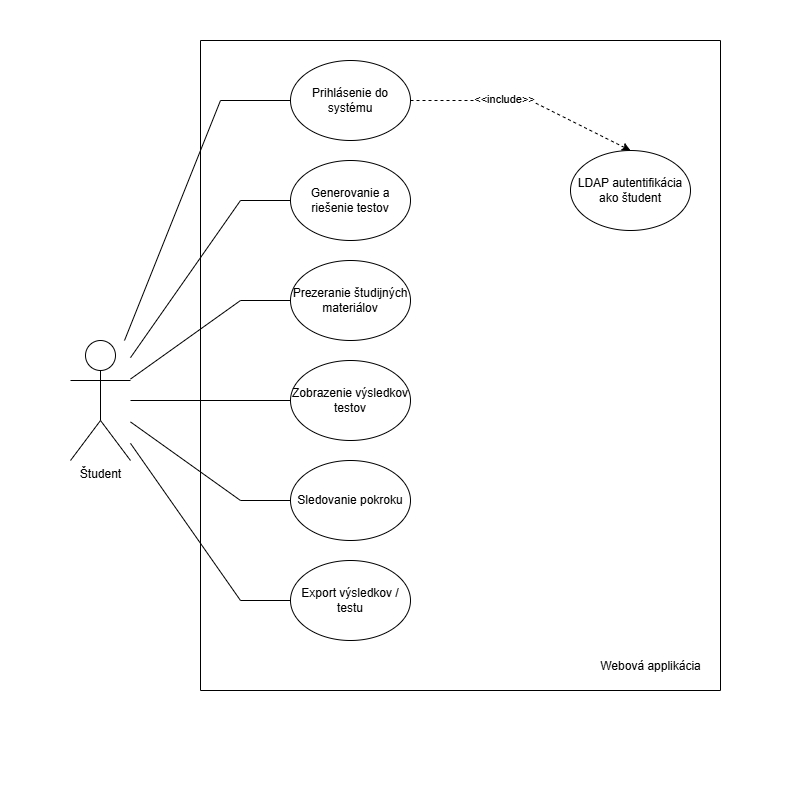
\includegraphics[width=16cm]{img/diagram_student.png}
  \caption{Diagram prípadov použitia pre študenta.}
  \label{studentdiagram}
\end{figure}



\subsubsection{Diagramy prípadov použitia pre administrátora}
\begin{figure}[H]
  \centering
  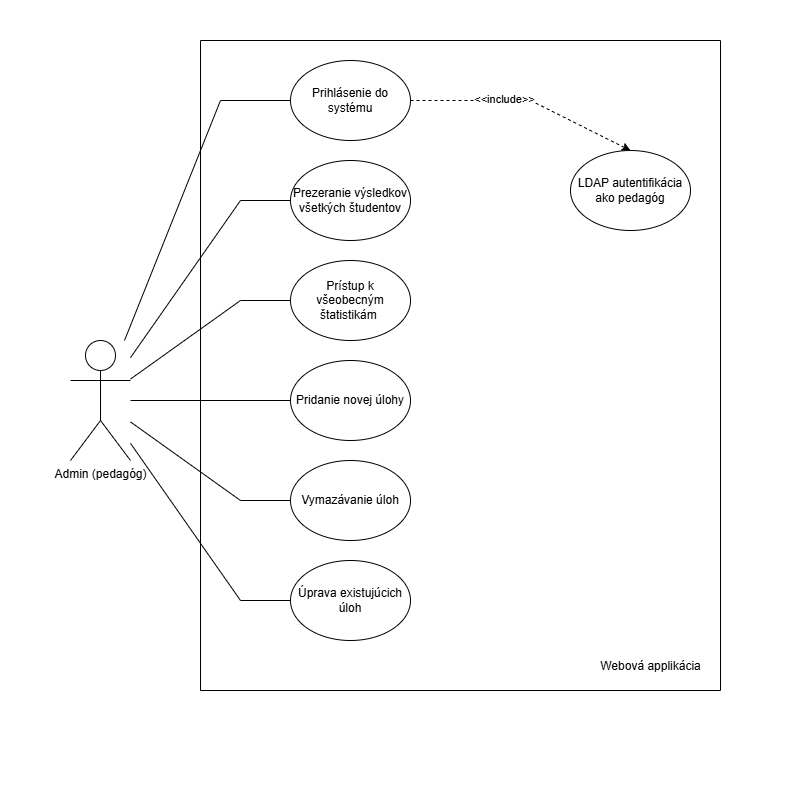
\includegraphics[width=16cm]{img/diagram_admin.png}
  \caption{Diagram prípadov použitia pre administrátora.}
  \label{admindiagram}
\end{figure}



 \subsection{Databáza}
 Databázovým systémom našej webovej aplikácie je PostgreSQL, ktorý sme si zvolili pre jeho flexibilnú prácu s dátami. 
 Využívame najmä podporu pre JSONB, ktorá nám umožňuje efektívne ukladať a vyhľadávať polostruktúrované dáta, ako sú odpovede či nápovedy.

Ďalšou výhodou je podpora poľových typov (ARRAY), ktoré zjednodušujú štruktúru databázy tým, že umožňujú uchovávať viacero hodnôt v jednom stĺpci. 
PostgreSQL nám tak poskytuje výkonné a praktické riešenie pre prácu s komplexnými údajmi.

Na obrázku č~\ref{dbtableobr}. je zobrazený logický ER diagram (Entity-Relationship Diagram) databázového modelu našej aplikácie.
 Tento diagram zobrazuje vzťahy medzi jednotlivými entitami a znázorňuje, ako sú údaje v databáze navzájom prepojené.
\begin{figure}[htbp]
  \centering
  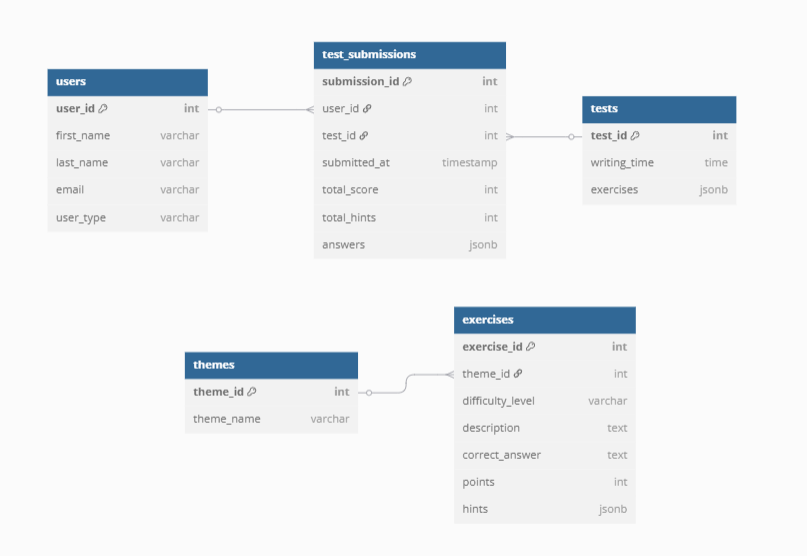
\includegraphics[width=12cm]{img/dbtablefinal.png}
  \caption{Logický ER diagram (Entity-Relationship Diagram) databázového modelu.}
  \label{dbtableobr}
\end{figure} 


Databáza sa skladá z nasledovných tabuliek:
\begin{itemize}
  \item \textit{users} – uchováva informácie o prihlásených používateľoch. 
  Keďže autentifikáciu zabezpečujeme prostredníctvom akademického LDAP systému, neukladáme žiadne citlivé dáta, ktoré by neboli dostupné priamo z \acrshort{ldap}. 
  Okrem základných údajov rozlišujeme aj typ používateľa (študent alebo administrátor/učiteľ), ktorý taktiež získavame z \acrshort{ldap} a ktorý ovplyvňuje rozsah oprávnení v aplikácii.
  \item \textit{themes} - obsahuje zoznam matematických tém, primárne z oblasti matematickej štatistiky, ktoré slúžia na kategorizáciu úloh.
  \item \textit{exercises} - uchováva údaje o jednotlivých úlohách, ako sú zadanie, úroveň obtiažnosti, počet bodov, správna odpoveď a dostupné nápovedy. 
  Každá úloha je priradená k jednej tematickej oblasti (theme\_id).
  \item \textit{tests} - reprezentuje sadu úloh, ktorá sa skladá z kombinácie úloh z databázy a automaticky generovaných úloh. Zároveň obsahuje aj časový limit na vypracovanie testu.
  \item \textit{test\_submissions} -  zaznamenáva konkrétne podania testov jednotlivými používateľmi.
   Obsahuje informácie o tom, kto test riešil, akú testovú sadu dostal, kedy test odovzdal, aké odpovede zadal, koľko bodov získal a koľko nápoved použil.
\end{itemize}

Polia \textit{answers} a \textit{hints} sú uložené vo formáte JSONB, čo umožňuje flexibilne uchovávať komplexné štruktúry dát, ako napríklad zoznam odpovedí alebo počty použitých nápoved ku konkrétnym úlohám.
 Príklad zápisu JSON dát v tomto stĺpci je znázornený na obrázku č.~\ref{dbjsonb}.

 \begin{figure}[h!]
  \centering
  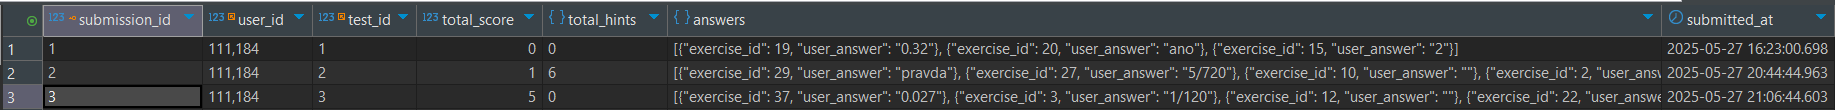
\includegraphics[width=\textwidth]{img/dbjsonb.png}
  \caption{Príklad zápisu JSON dát v stĺpci \textit{answers}.}
  \label{dbjsonb}
 \end{figure}

 Každé zadanie úlohy (description) je uložené ako reťazec vo formáte LaTeX, čo umožňuje pohodlný zápis matematických vzorcov a výrazov. Tento spôsob zápisu je výhodný najmä pre potreby zobrazovania úloh vo webovom rozhraní pomocou renderovacích nástrojov ako je napríklad MathJax, ktoré dokážu LaTeX premeniť na kvalitne vykreslené rovnice.

Príklad zápisu jednej úlohy s použitím LaTeX zápisu je znázornený na obrázku č.~\ref{latexpriklad}.

\begin{figure}[H]
  \centering
  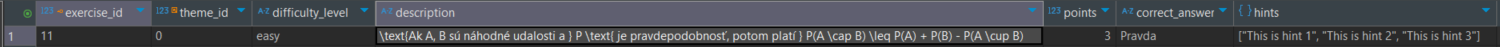
\includegraphics[width=\textwidth]{img/latex_example.png}
  \caption{Ukážka LaTeX zápisu zadania úlohy v databáze}
  \label{latexpriklad}
\end{figure}


\subsection{Použivateľské rozhranie}

Používateľské rozhranie aplikácie bolo navrhnuté s dôrazom na prehľadnosť, jednoduchosť a intuitívnu navigáciu, čím sa znižuje kognitívna záťaž používateľa a zvyšuje sa celková používateľská skúsenosť (UX). Cieľom návrhu bolo zabezpečiť, aby sa aj používateľ s minimálnymi digitálnymi zručnosťami dokázal v prostredí jednoducho orientovať a efektívne pracovať so všetkými funkciami aplikácie.

Základná štruktúra dizajnu bola vytvorená v nástroji Figma, ktorý umožnil vizuálny návrh používateľského rozhrania ešte pred samotnou implementáciou. Rozhranie je koncipované ako hlavné menu s veľkými, vizuálne výraznými blokmi, ktoré reprezentujú jednotlivé kľúčové funkcie aplikácie:
\begin{itemize} 
  \item Písanie testu 
  \item Zobrazenie napísaných testov 
  \item Export testov a výsledkov 
  \item Prístup k študijným materiálom 
\end{itemize}

Ako môžeme vidieť na obrázku č.~\ref{homescreen}, ide o hlavnú obrazovku aplikácie, ktorá slúži ako východiskový bod pre všetky hlavné činnosti používateľa.

\begin{figure}[h!]
  \centering
  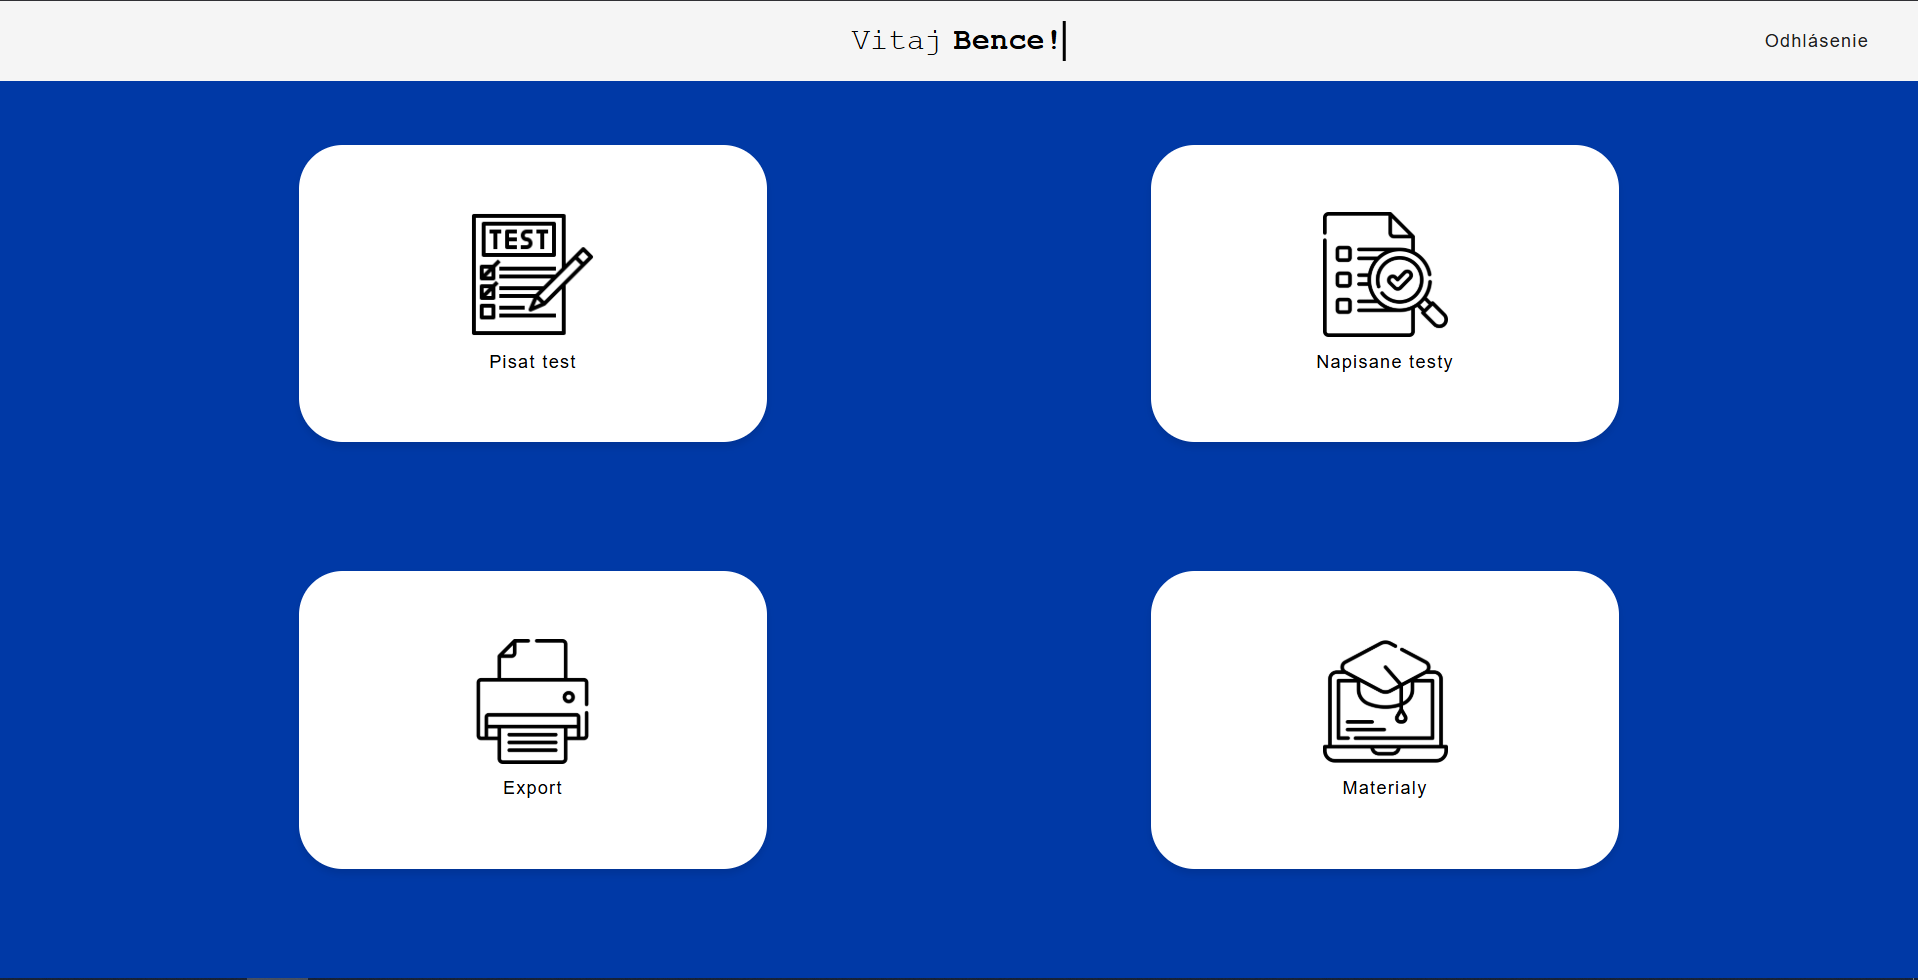
\includegraphics[width=16cm]{img/homepage.png}
  \caption{Hlavná obrazovka aplikácie.}
  \label{homescreen}
\end{figure} 

Navigácia v aplikácii je zabezpečená pomocou horného navigačného panela, ktorý obsahuje možnosť návratu na hlavnú obrazovku a tlačidlo pre odhlásenie zo systému. Tento prvok je dostupný na všetkých podstránkach aplikácie, čím sa zabezpečuje jednotný a konzistentný spôsob navigácie naprieč celým systémom.

Na obrázku č.~\ref{figmavizual} je zobrazený výrez z konceptuálneho návrhu podstránky \textit{Písať test}, ktorý bol súčasťou úvodného vizuálneho návrhu. V porovnaní s finálnou implementáciou prešli niektoré prvky úpravami zameranými na lepšiu prehľadnosť, responzívnosť a používateľskú použiteľnosť.

\begin{figure}[H]
  \centering
  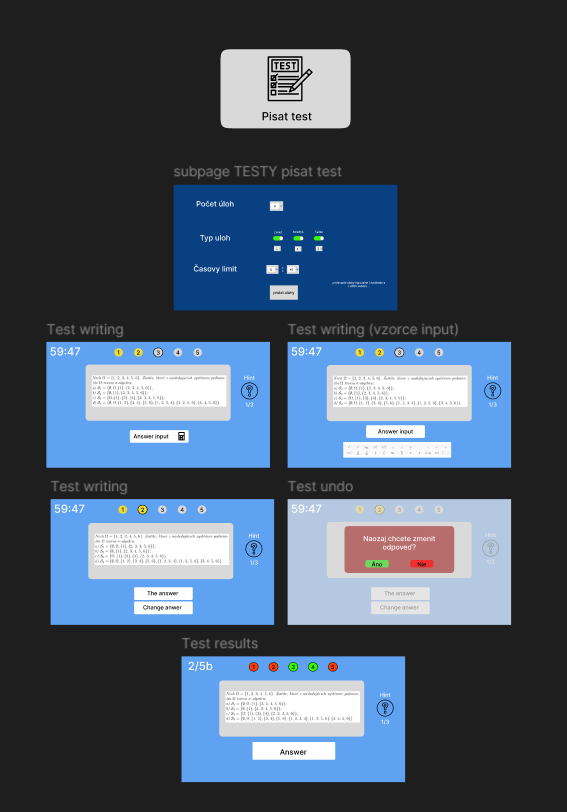
\includegraphics[width=16cm]{img/figma_screen.png}
  \caption{Výrez z konceptuálneho návrhu podstránky Písať test.}
  \label{figmavizual}
\end{figure} 

\subsection{Preskúšanie sa}

Súčasťou navrhovanej webovej aplikácie je stránka umožňujúca používateľom vytvárať vlastné testovacie sady úloh na precvičenie a preverenie vedomostí z oblasti pravdepodobnosti a štatistiky.
 Používateľské rozhranie tejto stránky (obrázok~\ref{test-creation}) bolo navrhnuté tak, aby bolo intuitívne a aby zabezpečovalo príjemnú používateľskú skúsenosť (UX).

\begin{figure}[h!]
  \centering
  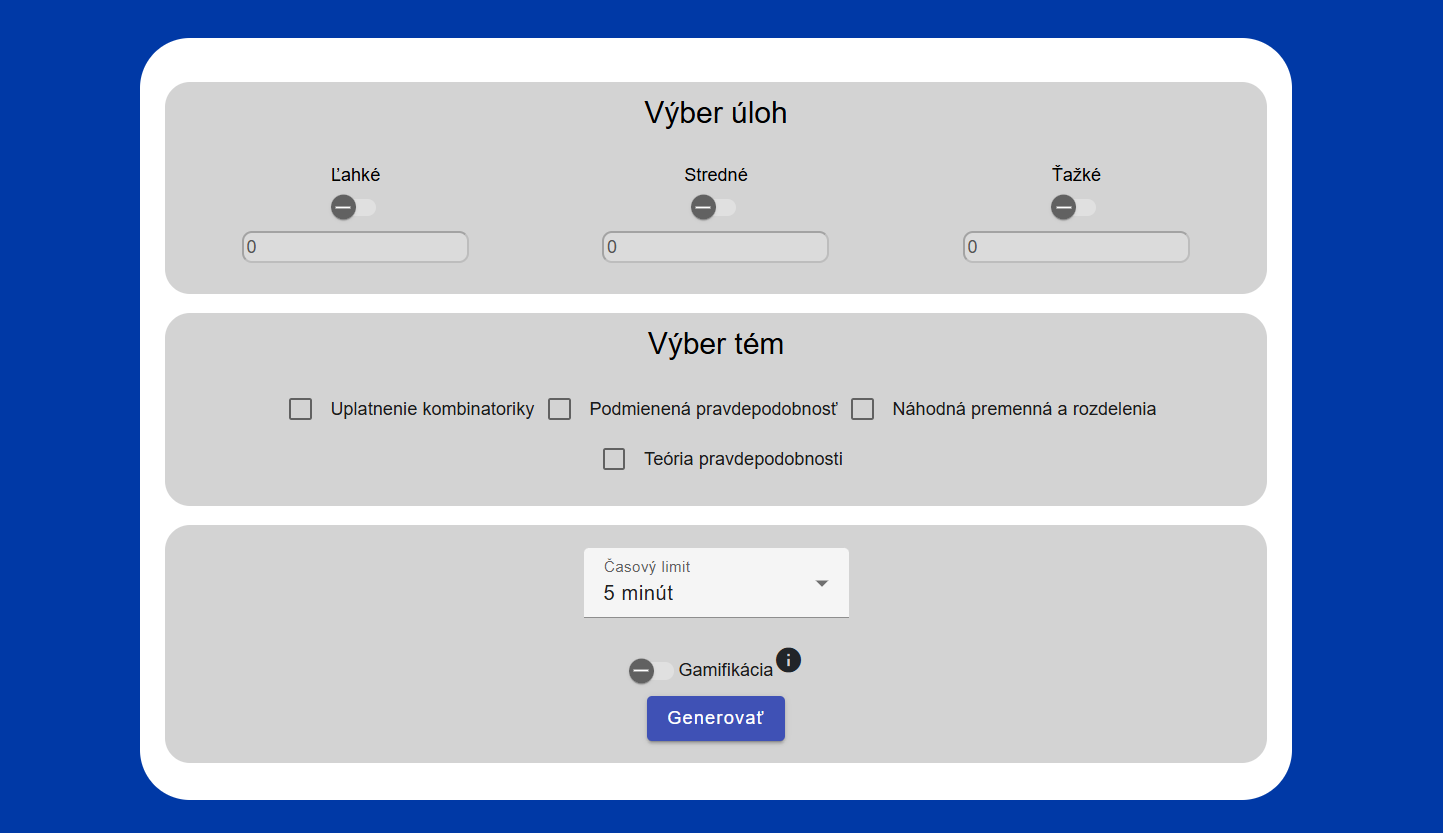
\includegraphics[width=14cm]{img/test-creation.png}
  \caption{Používateľské rozhranie stránky pre vytvorenie testovacej sady.}
  \label{test-creation}
\end{figure}

Na tejto stránke má používateľ možnosť presne definovať parametre generovaného testu, ako napríklad:

\begin{itemize}
  \item \textbf{Výber tém} – používateľ si môže označiť matematické témy, z ktorých chce byť testovaný. Ide najmä o témy ako pravdepodobnosť a rozdelenia, štatistika a analýza dát, kombinatorika a teória množín, a tiež aplikácie a reálne scenáre.
  \item \textbf{Typ a obtiažnosť úloh} – umožňuje nastaviť počet ľahkých, stredne ťažkých a ťažkých úloh.
  \item \textbf{Časový limit} – určuje maximálny čas na vypracovanie celého testu.
  \item \textbf{Gamifikácia} – voliteľná funkcionalita, ktorej účelom je zvýšiť motiváciu používateľov prostredníctvom herných prvkov, bližšie vysvetlená v nasledujúcej podkapitole.
\end{itemize}

Po úspešnom vygenerovaní testovej sady je používateľ automaticky presmerovaný na stránku samotného preskúšania (obrázok~\ref{test-writing}). 
Pri návrhu tejto stránky sme kládli dôraz na vizuálnu spätnú väzbu pre používateľa – už zodpovedané úlohy sú jasne vizuálne označené, čím sa zlepšuje prehľadnosť testu. 
Súčasťou rozhrania je aj stručný popis používania aplikácie, ktorý sa zobrazí kliknutím na príslušnú ikonu s informáciami.

Po uplynutí časového limitu sa používateľovi automaticky zobrazí modálne okno, ktoré informuje o ukončení testu a odoslaní odpovedí na spracovanie a vyhodnotenie.

Na správne a čitateľné vykresľovanie matematických výrazov a rovníc bola použitá JavaScriptová knižnica \textbf{MathJax}.
 Tá zabezpečuje bezproblémové zobrazenie matematických symbolov a vzorcov priamo vo webovom prehliadači používateľa.
\begin{figure}[h!]
  \centering
  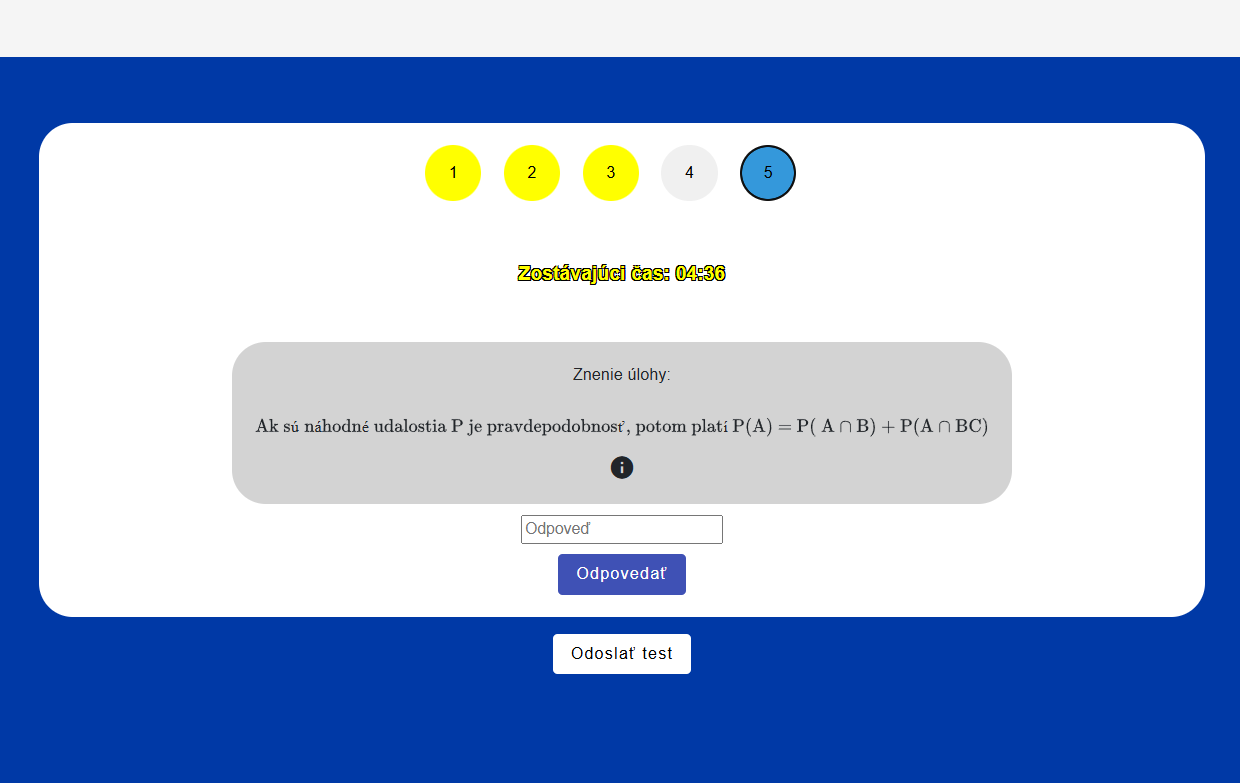
\includegraphics[width=14cm]{img/test-writing.png}
  \caption{Používateľské rozhranie stránky počas priebehu testu.}
  \label{test-writing}
\end{figure}



\subsubsection{Gamifikácia}

S cieľom zvýšiť atraktívnosť vzdelávacieho procesu a posilniť motiváciu študentov bola do aplikácie implementovaná \textbf{gamifikácia}, teda využitie herných prvkov v nehernom kontexte. 
Gamifikačné mechanizmy majú potenciál výrazne zlepšiť angažovanosť študentov, podporiť ich súťaživosť a vytvoriť pozitívne motivujúce prostredie na systematické precvičovanie vedomostí.

V rámci navrhnutej aplikácie sme zaviedli nasledujúce gamifikačné prvky:

\begin{itemize} \item \textbf{Percentilové hodnotenie} – namiesto klasického zoradenia používateľov podľa počtu bodov aplikácia využíva hodnotenie na základe \textbf{percentilu}. 
  Tento ukazovateľ vyjadruje, aké percento ostatných študentov dosiahlo horší alebo rovnaký výsledok.
   Zobrazenie percentilu poskytuje študentovi okamžitú a objektívnu informáciu o jeho relatívnej výkonnosti v rámci všetkých účastníkov testovania a zároveň ho motivuje k ďalšiemu zlepšovaniu.
  Ukážku zobrazovania percentilového hodnotenia možno vidieť na obrázku~\ref{test-results}.
  

\item \textbf{Bodový systém s bonusmi} – používateľ získava štandardné body za každú správne zodpovedanú otázku. 
Okrem toho sú prideľované aj bonusové body za rýchlosť odpovede, čím sa študenti podporujú v efektívnom a rýchlom riešení úloh.

\item \textbf{Vizuálna a zvuková spätná väzba} – aplikácia okamžite reaguje na správne alebo nesprávne odpovede študenta. Vizuálne je táto spätná väzba reprezentovaná farebným označením stavu jednotlivých otázok, pričom je doplnená aj vhodnými zvukovými efektmi. Týmto spôsobom dostáva používateľ jasnú a jednoznačnú informáciu o svojej aktuálnej úspešnosti.

\begin{figure}[h!]
  \centering
  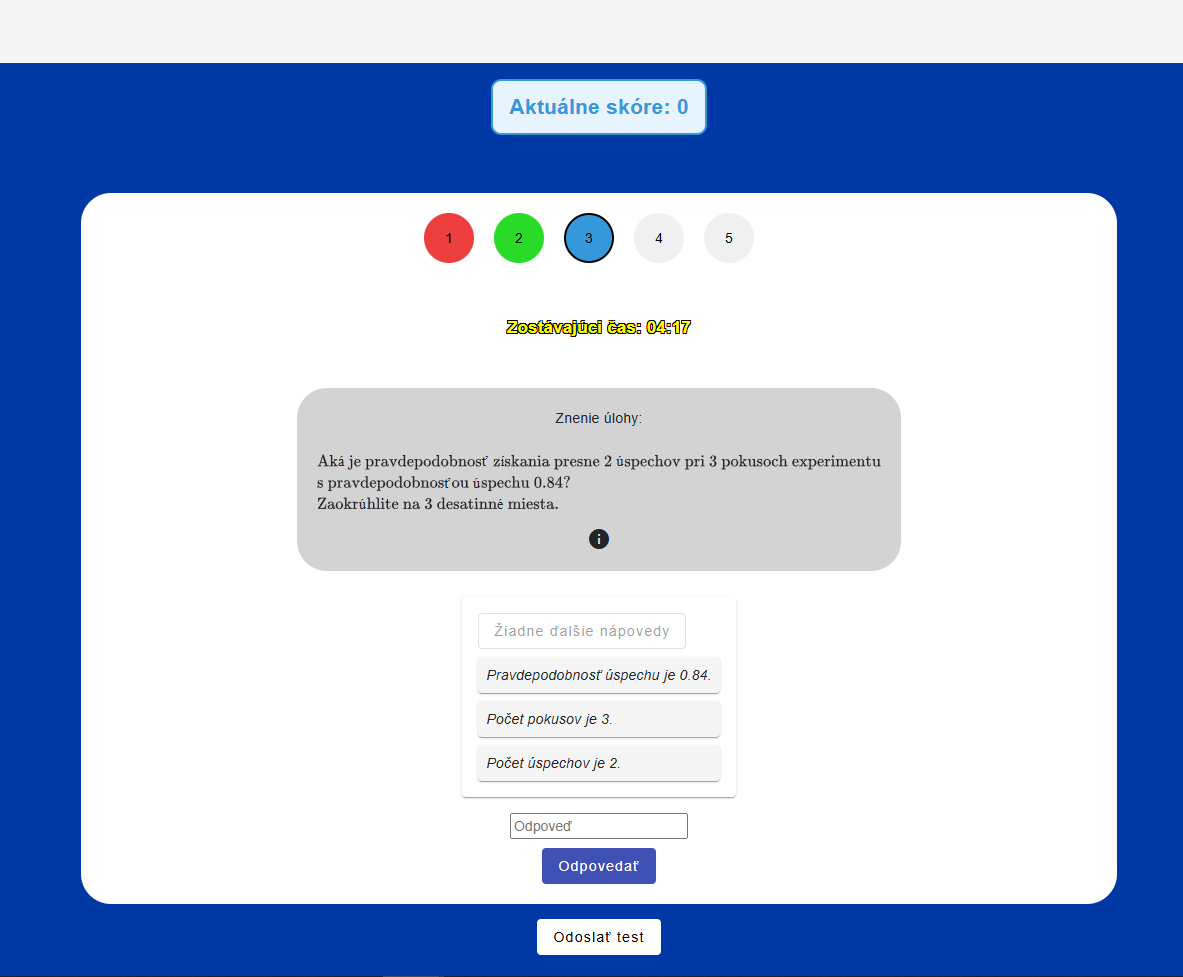
\includegraphics[width=14cm]{img/gamification.png}
  \caption{Ukážka vizuálnej spätnej väzby v gamifikovanom režime testovania.}
  \label{fig:gamification-feedback}
\end{figure}

Týmto spôsobom dostáva používateľ jasnú a jednoznačnú informáciu o svojej aktuálnej úspešnosti.

\item \textbf{Nápovedy s penalizáciou} – v prípade, že používateľ potrebuje pomôcť s riešením úloh, má možnosť využiť nápovedu. Tá ho môže nasmerovať k správnemu riešeniu, avšak za každú použitú nápovedu sú používateľovi odpočítané body. Týmto spôsobom podporujeme študentov k samostatnosti a zároveň pridávame do vzdelávania súťažný rozmer. \end{itemize}

Na stránke so štatistikami má študent následne možnosť vidieť, v akom percentile výkonnosti sa nachádza, čo mu poskytuje objektívnu informáciu o jeho relatívnej úspešnosti voči ostatným používateľom aplikácie. Tieto prvky spolu vytvárajú efektívne a interaktívne prostredie, ktoré podporuje kontinuálne vzdelávanie a rozvoj matematických schopností študentov.
\subsubsection{Generovanie úloh TODO}

Pri návrhu aplikácie sme sa rozhodli implementovať mechanizmus \textbf{automatického generovania úloh}, ktorého cieľom bolo zvýšiť variabilitu testov a zabezpečiť, aby používatelia neboli limitovaní iba na statické úlohy uložené v databáze. 
Takto generované úlohy pridávajú do testovania prvok náhodnosti a prekvapenia, čím dochádza k efektívnejšiemu prevereniu skutočných vedomostí a schopností študenta.
\subsection{Materialy}
Ďalšou súčasťou aplikácie je sekcia študijných materiálov, ktorá slúži študentom ako efektívna podpora počas štúdia matematickej štatistiky a pravdepodobnosti. 
Táto časť aplikácie obsahuje systematicky usporiadané študijné poznámky, ktoré pokrývajú učebné osnovy predmetu Matematická štatistika.
 Obsah je kategorizovaný podľa jednotlivých tematických oblastí, čo umožňuje jednoduchú orientáciu v študovanom obsahu.

Každá téma obsahuje teoretické poznatky spolu s jasne spracovanými vzorovými príkladmi. 
Súčasťou týchto príkladov je aj detailný postup výpočtu, ktorý študentom slúži ako metodická pomôcka pri riešení podobných úloh.

\begin{figure}[H]
  \centering
  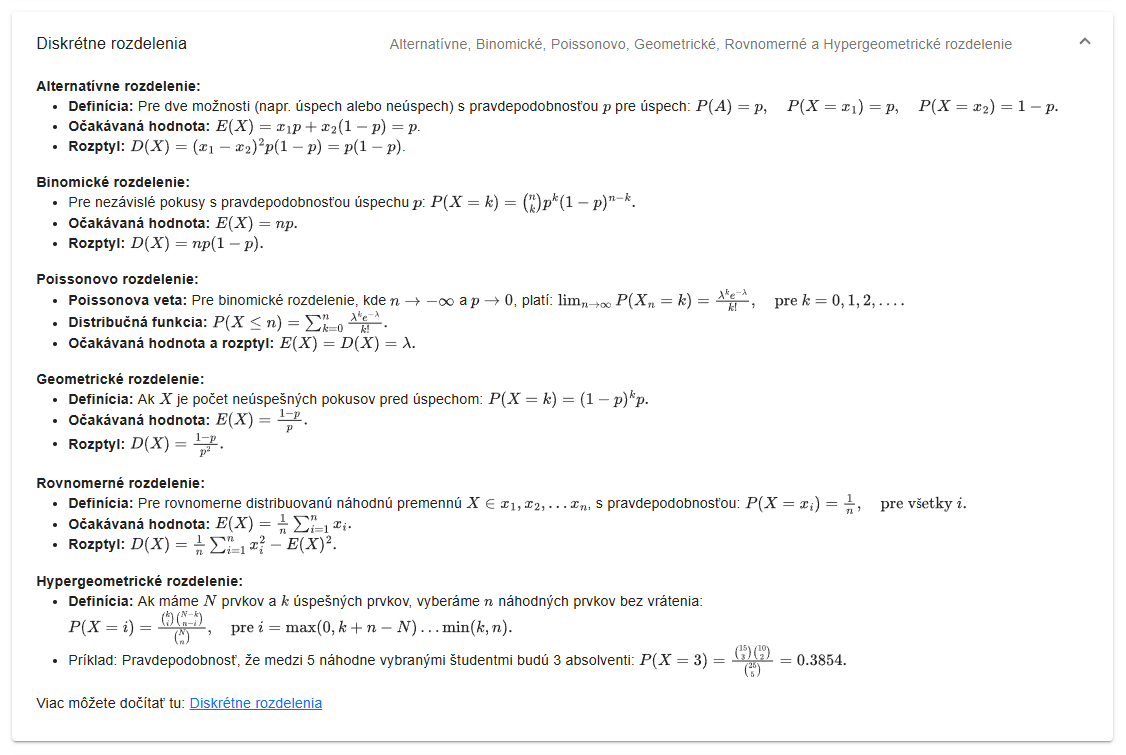
\includegraphics[width=14cm]{img/materialy.png}
  \caption{Ukážka sekcie študijných materiálov s príkladom.}
  \label{materialy}
  \end{figure}

\subsubsection{Interaktivne grafy}
Na zvýšenie interaktivity a pochopenia zložitých matematických konceptov sú v rámci materiálov integrované aj interaktívne grafy. 
Tieto grafy vizuálne demonštrujú dôležité pravdepodobnostné princípy, ako napríklad priebehy distribučných funkcií alebo hustoty pravdepodobnosti rôznych rozdelení. 
Grafické znázornenie výrazne uľahčuje študentom pochopenie abstraktných matematických myšlienok a prehlbuje ich schopnosť aplikovať získané vedomosti v praxi.
\begin{figure}[H]
  \centering
  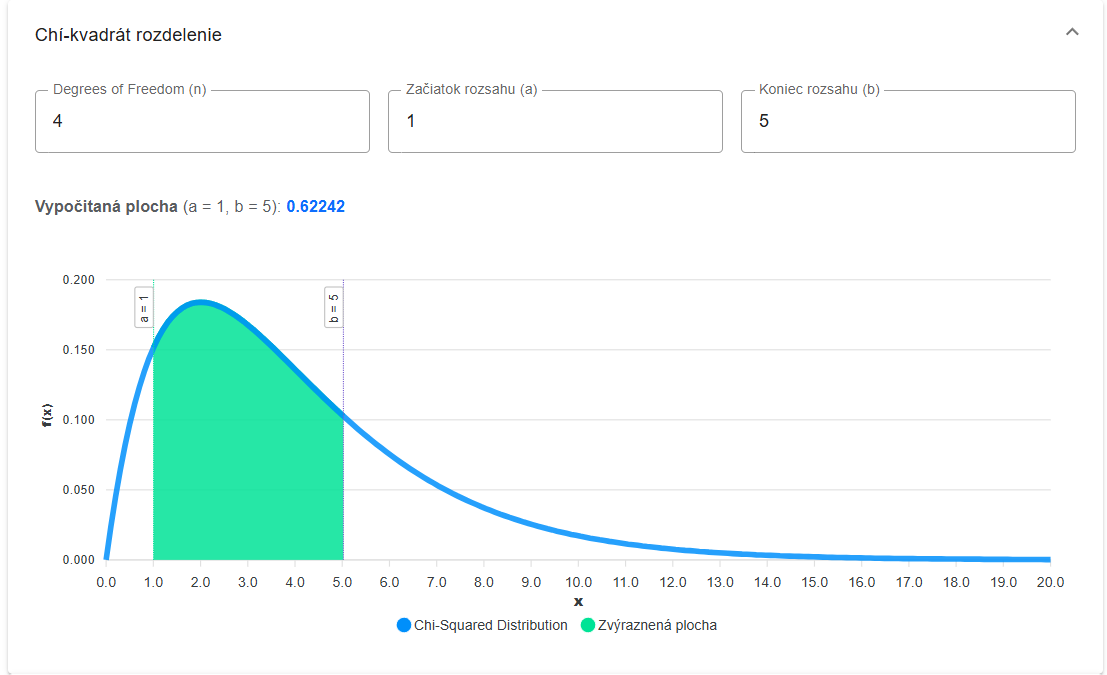
\includegraphics[width=14cm]{img/grafy.png}
  \caption{Ukážka interaktívneho grafu.}
  \label{grafy}
  \end{figure}

\subsection{Vyhodnocovanie úloh}

Po dokončení testu má používateľ k dispozícii detailný rozbor svojho riešenia. 
Na tejto podstránke je možné spätne prehliadať absolvované testy, pričom ku každému testu je zobrazovaný zoznam jednotlivých úloh s vyznačením správnosti odpovede.

 Každú úlohu je možné rozkliknúť a prezrieť si zadanie spolu s odpoveďou, čo podporuje proces spätného učenia a upevňovania vedomostí.

Okrem samotného zoznamu úloh je súčasťou zobrazenia aj základné štatistické zhrnutie testu, ako napríklad počet správnych odpovedí, celkový počet získaných bodov a dosiahnutý percentil.

Percentil poskytuje používateľovi okamžitú informáciu o jeho relatívnom postavení medzi všetkými účastníkmi testovania, a to na základe získaného skóre.


\begin{figure}[H]
  \centering
  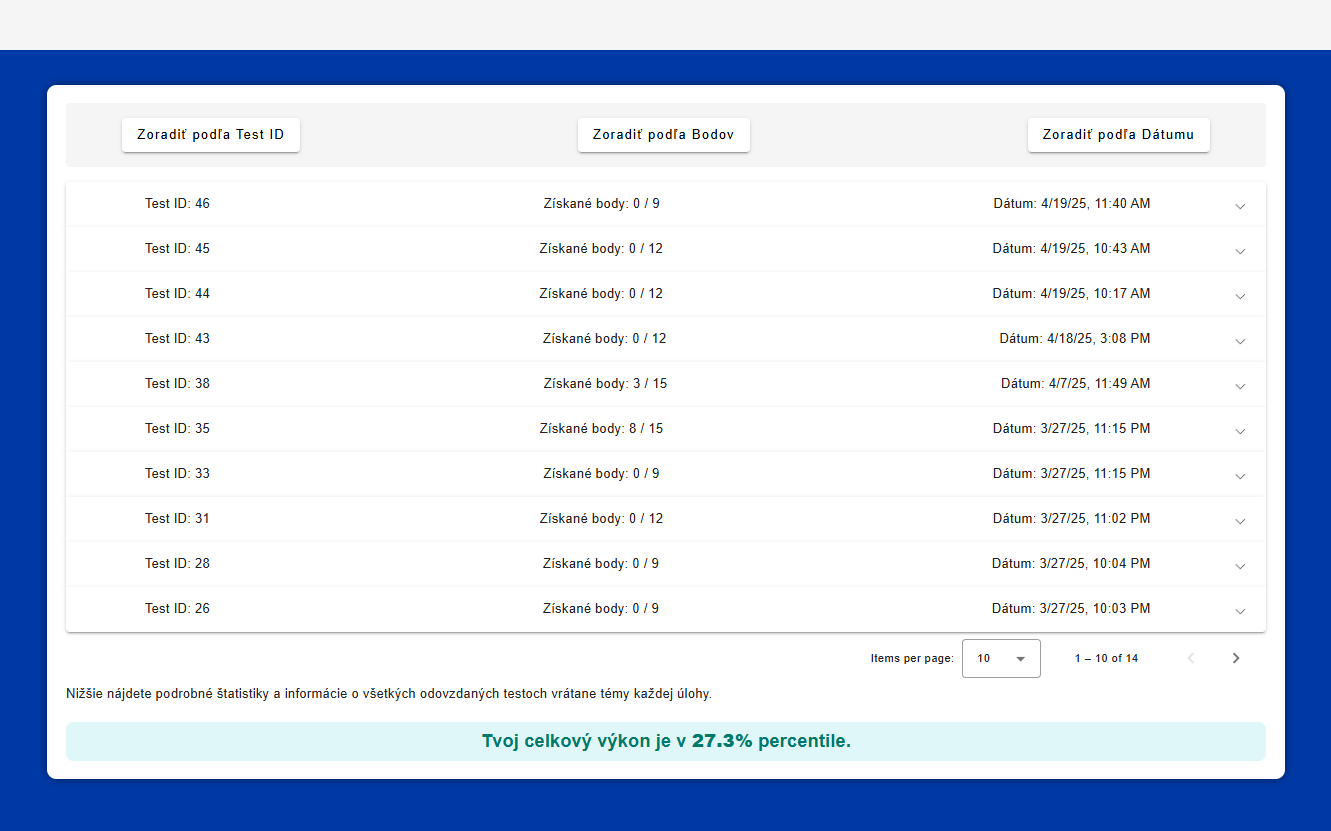
\includegraphics[width=14cm]{img/test-results.png}
  \caption{Ukážka podstránky vyhodnocovania testu a zobrazenie dosiahnutého percentilu.}
  \label{test-results}
\end{figure}



\subsection{Vytváranie a úprava úloh administrátorom TODO: Fotka mozno}

V rámci administrátorskej časti aplikácie bola implementovaná funkcionalita umožňujúca správcom systému vytvárať nové úlohy a upravovať existujúce zadania.
 Cieľom tejto funkcionality je umožniť dynamické rozširovanie databázy úloh bez potreby manuálnych zásahov do databázy na úrovni servera.

Pri návrhu rozhrania na vkladanie úloh bolo dôležité zabezpečiť, aby bol proces tvorby matematických otázok intuitívny a používateľsky prívetivý, najmä pri práci s matematickými zápismi a vzorcami.
 Tento cieľ bol dosiahnutý integráciou knižnice \textbf{MathQuill}, ktorá umožňuje dynamické a interaktívne zadávanie matematických výrazov.

\textbf{MathQuill} poskytuje rozhranie, v ktorom môže administrátor zadávať matematické vzorce v LaTeX formáte. 
V reálnom čase dochádza k ich prekladu do vizuálne čitateľnej podoby, čím sa zabezpečuje okamžitá spätná väzba a minimalizácia syntaktických chýb.
 Matematické výrazy sú zobrazované v editovateľnom textovom poli, ktoré verne imituje klasickú matematickú notáciu, čo výrazne zvyšuje používateľský komfort a presnosť zadávania úloh.

Táto funkcionalita nielen zjednodušuje proces tvorby úloh, ale zároveň zabezpečuje, že všetky matematické zápisy budú správne interpretované pri zobrazovaní úloh študentom v testoch a materiáloch.




 \section{Implementacia webovej aplikacie}
 V tejto kapitole sa podrobne venujeme implementačnej časti webovej aplikácie, pričom rozdeľujeme jednotlivé aspekty systému na backend, frontend a databázovú vrstvu.
  Cieľom tejto časti je ukázať, ako boli teoretické návrhy z predchádzajúcej kapitoly pretavené do konkrétnej technickej realizácie.

 V jednotlivých sekciách prezentujeme použité technológie a knižnice, ako aj konkrétne časti zdrojového kódu ilustrujúce dôležité funkcionality, 
 ako napríklad generovanie úloh, vizualizácie dát pomocou grafov alebo spracovanie používateľského vstupu pri pridávaní nových otázok do databázy.

 \subsection{Vývojové prostredie a inštalácia závislostí}

 Počas vývoja webovej aplikácie sme využívali vývojové prostredie \textbf{Visual Studio Code}\cite{vscode}, ktoré poskytuje množstvo rozšírení vhodných pre vývoj v JavaScripte a TypeScripte, ako aj nástroje na efektívnu správu projektovej štruktúry, ladenie a kontrolu syntaxe.
 
 Backendová časť aplikácie bola postavená na platforme \textbf{Node.js}, ktorá umožňuje spúšťanie JavaScriptového kódu na strane servera. Na správu knižníc a závislostí sme používali \acrfull{npm}, ktorý je súčasťou štandardnej inštalácie Node.js. 
 Pomocou neho boli do projektu inštalované všetky potrebné knižnice, ako napríklad \texttt{express}, \texttt{MathQuill}, \texttt{body-parser}, \texttt{cors} a ďalšie.
  
 Závislosti boli definované v súbore \texttt{package.json}, ktorý slúži zároveň ako dokumentačný a konfiguračný súbor pre projekt. Samotná inštalácia všetkých závislostí sa vykoná príkazom:
 
 \begin{verbatim}
 npm install
 \end{verbatim}
 
 Týmto príkazom sa automaticky stiahnu všetky knižnice uvedené v súbore \texttt{package.json} a pripravia sa na použitie v projekte.
 
 \subsection{Frontend – Angular}

Frontendová časť aplikácie bola implementovaná pomocou frameworku \textbf{Angular}, ktorý je postavený na TypeScripte a poskytuje robustnú architektúru pre budovanie komplexných single-page aplikácií (SPA).
 Angular ponúka množstvo výhod ako je komponentovo orientovaný vývoj, dvojcestná väzba dát, modulárnosť a rozsiahla komunita s kvalitnou dokumentáciou.

\bigskip
Na to, aby sme mohli Angular používať, je potrebné mať nainštalovaný \textbf{Node.js} a s ním aj správcu balíkov \acrshort{npm}, ktoré sme spomínali v predchádzajúcej sekcii. 
Po ich nainštalovaní je možné Angular \acrshort{cli} nainštalovať globálne\footnote{Prepínač \textit{-g} znamená globálnu inštaláciu, čím získame prístup ku príkazu \textit{ng} v ktoromkoľvek priečinku systému.}
pomocou príkazu:

\begin{verbatim}
npm install -g @angular/cli
\end{verbatim}

Správnu inštaláciu Angularu môžeme overiť pomocou príkazu:

\begin{verbatim}
ng version
\end{verbatim}

Výstup z tohto príkazu zobrazí verziu Angular \acrshort{cli}, ako aj verzie jednotlivých komponentov Angularu. Na obrázku~\ref{fig:ng-version} je znázornený výstup z tohto príkazu v termináli\footnote{Terminál vo Visual Studio Code predstavuje integrované rozhranie pre prácu s príkazovým riadkom priamo v editore.}.

\begin{figure}[H]
  \centering
  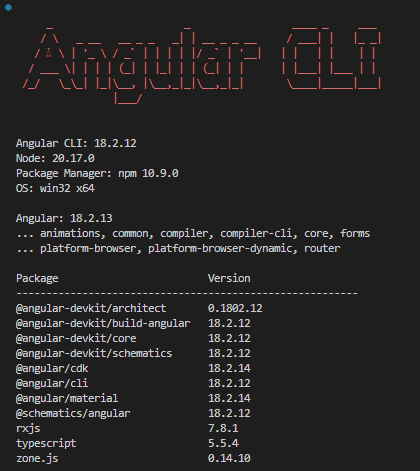
\includegraphics[width=10cm]{img/ng-version.png}
  \caption{Výstup príkazu \texttt{ng version} v termináli.}
  \label{fig:ng-version}
\end{figure}

\bigskip
Nový Angular projekt môžeme vytvoriť pomocou príkazu:

\begin{verbatim}
ng new angular-app
\end{verbatim}

Tento príkaz vygeneruje základnú adresárovú štruktúru aplikácie, vrátane konfiguračných súborov, ako je napríklad \texttt{angular.json}, \texttt{package.json}, a priečinkov \texttt{src/}, \texttt{app/} a ďalších. Po úspešnom vytvorení projektu môžeme aplikáciu spustiť príkazom:

\begin{verbatim}
ng serve
\end{verbatim}

Týmto príkazom sa automaticky nainštalujú všetky závislosti zo súboru \texttt{package-lock.json} a vytvorí sa priečinok \texttt{node\_modules}, ktorý obsahuje všetky knižnice potrebné na beh aplikácie.
 Aplikácia je následne dostupná na adrese \texttt{http://localhost:4200}.

Na obrázku~\ref{fig:angular-structure} je znázornená základná adresárová štruktúra Angular projektu po vytvorení.

\begin{figure}[H]
  \centering
  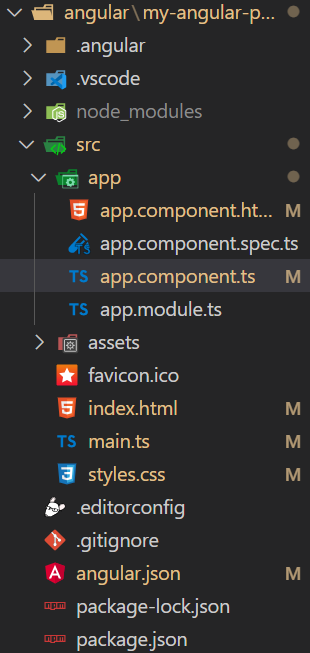
\includegraphics[width=6cm]{img/angular-structure.png}
  \caption{Základná štruktúra Angular projektu.}
  \label{fig:angular-structure}
\end{figure}

\subsubsection{Graficka cast tejto PICOVINY}
TODO
 RxJS
 node-sass kvoli renderovaniu
 apex charts - lazy loading
 math jax 
 chart.js 
 mathquill
 jQuery
 pdfmake
 Bootstrap
 bootstrap animation
 freedsound.org

\subsection{Backend}

 TODO
 Node
 Nginx

 CURL veci

 \paragraph{Inštalácia a použitie Express frameworku}

Inštalácia Expressu je jednoduchá a vykonáva sa pomocou balíčkovacieho nástroja \acrshort{npm} príkazom:

\begin{verbatim} npm install express \end{verbatim}

Po úspešnej inštalácii je možné vytvoriť základný server a definovať vlastné API routy. Najjednoduchšia implementácia servera môže vyzerať nasledovne:

\begin{lstlisting}[ caption={Ukážka základnej konfigurácie Express.js servera}, label={lst:basic-express-server}, language=java, style=code-listing ] 
  const express = require('express'); 
  const app = express(); 
  const port = 3000;

app.listen(port, () => { console.log(Server beží na porte ${port}); }); 
\end{lstlisting}

Tento server môžeme spustiť cez terminál pomocou príkazu:

\begin{verbatim} node server.js \end{verbatim}

kde \texttt{server.js} je názov súboru obsahujúceho uvedený kód. Ak je server úspešne spustený, v konzole sa vypíše správa \uv{Server beží na porte 3000}.
 V projekte je logika rozdelená do tzv. \textbf{servisných tried} (services), ktoré abstrahujú jednotlivé domény funkcionality – napríklad práca s testami, používateľmi alebo štatistikami. 
 Tieto triedy slúžia ako rozhranie medzi routou a databázovou logikou. 
Na obrázku~\ref{fig:backend-services} je znázornený výrez zo štruktúry backendu so zameraním na jednotlivé služby.

Tento kód vytvorí základný server, ktorý je pripravený na ďalšie definovanie rout a pridávanie funkcionality.
 V projekte je logika rozdelená do tzv. \textbf{servisných tried} (services), ktoré abstrahujú jednotlivé domény funkcionality.
  Tieto triedy slúžia ako rozhranie medzi routou a databázovou logikou.
 Na obrázku~\ref{fig:backend-services} je znázornený výrez zo štruktúry backendu so zameraním na jednotlivé služby.
\begin{figure}[H]
  \centering
  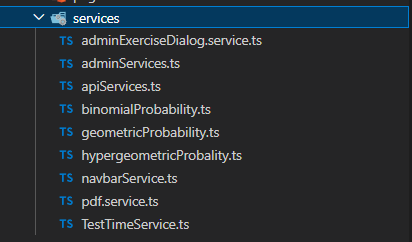
\includegraphics[width=13cm]{img/backend-services.png}
  \caption{Ukážka štruktúry backendových služieb v aplikácii.}
  \label{fig:backend-services}
\end{figure}

\bigskip
Na to, aby frontend mohol komunikovať s backendom, je potrebné povoliť prístup medzi rôznymi doménami (napr. frontend beží na \texttt{http://localhost:4200} a backend na \texttt{http://localhost:3000}). Na tento účel sme použili knižnicu \textbf{CORS} (\textit{Cross-Origin Resource Sharing}), ktorá bola nakonfigurovaná nasledovne:

\begin{lstlisting}[
  caption={Konfigurácia CORS pre komunikáciu medzi FE a BE},
  label={lst:cors-config},
  language=java,
  style=code-listing
]
const cors = require('cors');
app.use(cors({
  origin: 'http://localhost:4200',
  credentials: true
}));
\end{lstlisting}

Bez tejto konfigurácie by prehliadač blokoval požiadavky medzi rôznymi portmi alebo doménami, čo by znemožnilo komunikáciu medzi frontendom a backendom.

\bigskip
Na správne spracovanie dát typu \texttt{application/json}, ktoré odosiela Angular prostredníctvom POST alebo PUT požiadaviek, sme použili middleware \textbf{body-parser}. Tento middleware zabezpečí, že JSON objekt v tele požiadavky bude automaticky spracovaný a dostupný cez \texttt{req.body}. Je to obzvlášť dôležité pri práci s databázou PostgreSQL, kde používame dátový typ \texttt{JSONB}.

\begin{lstlisting}[
  caption={Použitie body-parser pre spracovanie JSON požiadaviek},
  label={lst:body-parser},
  language=java,
  style=code-listing
]
const bodyParser = require('body-parser');
app.use(bodyParser.json());
\end{lstlisting}

Týmto nastavením zabezpečíme, že každý JSON payload zo strany klienta bude backendom správne spracovaný a následne uložený do databázy vo formáte \texttt{JSONB}.


 \subsubsection{Autentifikácia}

 Prihlasovanie používateľov v aplikácii je riešené pomocou \textbf{LDAP autentifikácie}, pričom aplikácia komunikuje s akademickým LDAP serverom \texttt{ldap.stuba.sk}. Na overenie prihlasovacích údajov využívame knižnicu \texttt{ldap-authentication}, ktorá zabezpečuje jednoduché pripojenie a autentifikáciu voči vzdialenému LDAP serveru. Knižnica má ako závislosť \texttt{ldapjs}, ktorá realizuje nízkoúrovňovú komunikáciu.
 
 Samotná autentifikácia je realizovaná pomocou nasledovnej asynchrónnej funkcie:
 
 \begin{lstlisting}[
   caption={Funkcia na autentifikáciu používateľa cez LDAP},
   label={lst:ldap-auth},
   language=java,
   style=code-listing
 ]
 async function ldapAuth(username, password) {
   try {
     const options = {
       ldapOpts: { url: 'ldap://ldap.stuba.sk' },
       userDn: `uid=${username},ou=People,dc=stuba,dc=sk`,
       userPassword: password,
       userSearchBase: 'ou=People,dc=stuba,dc=sk',
       usernameAttribute: 'uid',
       username: username,
     };
 
     return await authenticate(options);
   } catch (error) {
     throw new Error('LDAP bind failed: ' + error.message);
   }
 }
 \end{lstlisting}
 
 Na strane backendu používame knižnicu \texttt{express-session}, ktorá nám umožňuje uchovávať informáciu o prihlásenom používateľovi v rámci session. Týmto spôsobom vieme zabezpečiť, že používateľ ostane prihlásený aj pri opakovanej návšteve stránky počas aktívnej relácie.
 
 Po úspešnej autentifikácii sa vytvorí zjednodušený objekt používateľa, ktorý sa uloží do databázy (ak ešte neexistuje), a zároveň sa uloží do session nasledovne:
 
 \begin{lstlisting}[
   caption={Spracovanie prihlasovania a uloženie používateľa do session},
   label={lst:login-session},
   language=java,
   style=code-listing
 ]
 app.post('/login', async (req, res) => {
   const { username, password } = req.body;
   try {
     const user = await ldapAuth(username, password);
     const processedUser = {
       userId: user.uisId,
       employeeType: user.employeeType,
       givenName: user.givenName,
       lastName: user.sn,
       email: user.mailLocalAddress[1],
     };
 
     // Insert into DB if new
     try {
       const existing = await db.findUserById(processedUser.userId);
       if (!existing) {
         await db.insertUser(processedUser);
       }
     } catch (dbErr) {
       console.error('DB error:', dbErr.message);
     }
 
     // Save user to session
     req.session.user = processedUser;
     res.status(200).json(processedUser);
   } catch (err) {
     res.status(401).json({ error: 'Authentication failed: ' + err.message });
   }
 });
 \end{lstlisting}
 
 \paragraph{Ochrana súkromných a administrátorských rout na strane frontendu}

Na strane klienta (v Angulari) využívame vlastný súbor \texttt{auth.guard.ts}, ktorý zabezpečuje, že k určitým stránkam aplikácie má prístup iba autentifikovaný používateľ. Tento guard je súčasťou smerovania (routing) a overuje, či existuje používateľ v úložisku \texttt{sessionStorage}. Ak nie, používateľ je automaticky presmerovaný na prihlasovaciu stránku.

Okrem toho tento guard podporuje aj kontrolu rolí používateľov. Pomocou atribútu \texttt{expectedEmployeeType} v definícii trasy vieme zabezpečiť, že niektoré stránky (napr. administrátorské) budú dostupné len používateľom s určitou rolou (napr. \texttt{admin}).

\begin{lstlisting}[
  caption={Implementácia AuthGuard v Angulari},
  label={lst:auth-guard},
  language=java,
  style=code-listing
]
canActivate(route: ActivatedRouteSnapshot, state: RouterStateSnapshot): boolean {
  const user = this.apiService.getUserFromStorage();

  if (!user) {
    this.router.navigate(['/']);
    return false;
  }

  const expectedEmployeeType = route.data['expectedEmployeeType'];
  if (expectedEmployeeType && user.employeeType !== expectedEmployeeType) {
    this.router.navigate(['/menu']);
    return false;
  }

  return true;
}
\end{lstlisting}

Definícia ciest sa nachádza v súbore \texttt{app-routing.module.ts}, kde sa pomocou \texttt{canActivate} zabezpečuje ochrana jednotlivých komponentov. Ako môžeme vidieť na príklade nižšie, každá trasa, ktorá vyžaduje prihlásenie, je chránená pomocou \texttt{AuthGuard}. Pre admin rozhrania je navyše špecifikovaný parameter \texttt{expectedEmployeeType}, čo zabezpečuje aj kontrolu oprávnení.

\begin{lstlisting}[
  caption={Definícia rout v Angulari s ochranou pomocou AuthGuard},
  label={lst:routing},
  language=java,
  style=code-listing
]
const routes: Routes = [
  { path: '', component: LoginModalComponent },
  { path: 'menu', component: MenuPageComponent, canActivate: [AuthGuard] },
  { path: 'test', component: TestCreationComponent, canActivate: [AuthGuard] },
  { path: 'stats', component: StatsPageComponent, canActivate: [AuthGuard] },
  { path: 'done', component: TestDoneComponent, canActivate: [AuthGuard] },
  { path: 'mats', component: MaterialsPageComponent, canActivate: [AuthGuard] },
  { path: 'test-writing', component: TestWritingComponent, canActivate: [AuthGuard] },
  { path: 'export', component: ExportPageComponent, canActivate: [AuthGuard] },
  { path: 'admin', component: AdminPageComponent, canActivate: [AuthGuard], data: { expectedEmployeeType: 'admin' } },
  { path: 'admin/statistics', component: AdminStatisticsComponent, canActivate: [AuthGuard], data: { expectedEmployeeType: 'admin' } },
  { path: '**', redirectTo: '' },
];
\end{lstlisting}

Týmto spôsobom zabezpečujeme na klientovi, že sa na súkromné alebo administrátorské stránky dostane iba oprávnený používateľ s platným session údajom, čím zvyšujeme bezpečnosť aplikácie.

 
 

 \subsubsection{Posielanie dat ????}
 tu napiseme o ApiService a o AdminService, a taktiez o autogenerovanych veciach ktore budu ale prepisane na helper servicky 

 
 \subsection{DB}
 prepajanie
  PostgreSQL
  built in mechanica pre data persistance and backps PostgreSQL allows you to specify a data directory where database files are stored, which you can mount as a volume or bind mount in Docker.****

  \subsection{Docker}
  single vs multiple container approach

  \section{Testovanie}